% /* vim: set filetype=tex: */
\documentclass{article}
\usepackage{amsmath}
\usepackage{color}
\usepackage{fancyvrb}
\usepackage{framed}
\definecolor{shadecolor}{RGB}{240,240,240}
%\DefineShortVerb[commandchars=\\\{\}]{\|}
\DefineVerbatimEnvironment{Highlighting}{Verbatim}{commandchars=\\\{\}}
% Add ',fontsize=\small' for more characters per line
\newenvironment{Shaded}{\begin{snugshade}}{\end{snugshade}}
%\newenvironment{Shaded}{}{}
\newcommand{\KeywordTok}[1]{\textcolor[rgb]{0.00,0.44,0.13}{\textbf{{#1}}}}
\newcommand{\DataTypeTok}[1]{\textcolor[rgb]{0.56,0.13,0.00}{{#1}}}
\newcommand{\DecValTok}[1]{\textcolor[rgb]{0.25,0.63,0.44}{{#1}}}
\newcommand{\BaseNTok}[1]{\textcolor[rgb]{0.25,0.63,0.44}{{#1}}}
\newcommand{\FloatTok}[1]{\textcolor[rgb]{0.25,0.63,0.44}{{#1}}}
\newcommand{\CharTok}[1]{\textcolor[rgb]{0.25,0.44,0.63}{{#1}}}
\newcommand{\StringTok}[1]{\textcolor[rgb]{0.25,0.44,0.63}{{#1}}}
\newcommand{\CommentTok}[1]{\textcolor[rgb]{0.38,0.63,0.69}{\textit{{#1}}}}
\newcommand{\OtherTok}[1]{\textcolor[rgb]{0.00,0.44,0.13}{{#1}}}
\newcommand{\AlertTok}[1]{\textcolor[rgb]{1.00,0.00,0.00}{\textbf{{#1}}}}
\newcommand{\FunctionTok}[1]{\textcolor[rgb]{0.02,0.16,0.49}{{#1}}}
\newcommand{\RegionMarkerTok}[1]{{#1}}
\newcommand{\ErrorTok}[1]{\textcolor[rgb]{1.00,0.00,0.00}{\textbf{{#1}}}}
\newcommand{\NormalTok}[1]{{#1}}

\setlength{\parindent}{0cm}
\usepackage[a4paper]{geometry}
\geometry{scale={0.80,0.85}}
\usepackage{booktabs}
\usepackage{longtable}
\usepackage{graphicx}
\setkeys{Gin}{width=.75\csname Gin@nat@width\endcsname,keepaspectratio}
\let\oldincludegraphics\includegraphics
\renewcommand\includegraphics[2][]{%
\begin{center}\oldincludegraphics[]{#2}\end{center}
}
\DeclareGraphicsExtensions{%
    .pdf,.PDF,%
    .png,.PNG,%
    .jpg,.mps,.jpeg,.jbig2,.jb2,.JPG,.JPEG,.JBIG2,.JB2}
\usepackage{floatrow}    
\renewcommand{\arraystretch}{1.2}
\usepackage{framed}

\usepackage[colorlinks=true,
linkcolor=blue]{hyperref}


\newcommand{\pkg}[1]{{\normalfont\fontseries{b}\selectfont #1}}
\let\proglang=\textsf
\let\code=\texttt

\title{The \textsf{lavaan} tutorial} 
\author{Yves Rosseel\\Department of Data Analysis\\%
  Ghent University (Belgium)}

\begin{document}
\maketitle
\begin{abstract}
If you are new to \pkg{lavaan}, this is the place to start. In this tutorial, we
introduce the basic components of lavaan: the model syntax, the fitting
functions (cfa, sem and growth), and the main extractor functions (summary,
coef, fitted, inspect). After we have provided two simple examples, we briefly
discuss some important topics: meanstructures, multiple groups, growth curve
models, mediation analysis, and categorical data. Along the way, we hope to
give you just enough information to get you started (but no more).
\end{abstract}

\tableofcontents

\section{Before you start}
Before you start, please read these points carefully:

\begin{itemize}
\item
  First of all, you must have a recent version ($3.0.0$ or higher) of R
  installed. You can download the latest version of R from this page:
  \url{http://cran.r-project.org/}.
\item
  The lavaan package is not finished yet. But it is already very useful
  for most users, or so we hope. However, some important features that
  are currently \emph{NOT} available in lavaan are:

  \begin{itemize}
  \item
    support for hierarchical/multilevel datasets (multilevel cfa,
    multilevel sem)
  \item
    support for discrete latent variables (mixture models, latent
    classes)
  \item
    Bayesian estimation
  \end{itemize}

  We hope to add these features in the next (two?) year(s) or so.
\item
  We consider the current version as \emph{beta} software. This does NOT
  mean that you can not trust the results. We believe the results are
  accurate. It does mean that things may change when new versions come
  out. For example, we may change the name of the arguments in function
  calls. And we change the internals of the source code constantly.
  However, the model syntax is fairly mature and has been stable for a
  while.
\item
  We do not expect you to be an expert in R. In fact, the lavaan package
  is designed to be used by users that would normally never use R.
  Nevertheless, it may help to familiarize yourself a bit with R, just
  to be comfortable with it. Perhaps the most important skill that you
  may need to learn is how to import your own datasets (perhaps in an
  SPSS format) into R. There are many tutorials on the web to teach you
  just that. Once you have your data in R, you can start specifying your
  model. We have tried very hard to make it as easy as possible for
  users to fit their models. Of course, if you have suggestions on how
  we can improve things, please let us know.
\item
  This document is written for first-time users of the lavaan package.
  It is not a reference manual, nor does it contain technical material
  on how things are done in the lavaan package. These documents are
  currently under preparation.
\item
  The lavaan package is free open-source software. This means (among
  other things) that there is no warranty whatsoever.
\item
  If you need help, you can ask questions in the lavaan discussion
  group. Go to \url{https://groups.google.com/d/forum/lavaan/} and join
  the group. Once you have joined the group, you can email your
  questions to
  \href{mailto:lavaan@googlegroups.com}{lavaan@googlegroups.com}. If you
  think you have found a bug, or if you have a suggestion for
  improvement, you can either email me directly (to alert me), post it
  to the discussion group (to discuss it), or open an issue on github
  (see \url{https://github.com/yrosseel/lavaan/issues}). The latter is
  useful once we have agreed it is a bug, and it should be fixed. If you
  report a bug, it is always very useful to provide a reproducible
  example (a short R script and some data).
\end{itemize}

\section{Installation of the package}
Since May 2010, the lavaan package is available on CRAN. Therefore, to
install lavaan, simply start up R, and type:

\begin{Shaded}
\begin{Highlighting}[]
\KeywordTok{install.packages}\NormalTok{(}\StringTok{"lavaan"}\NormalTok{, }\DataTypeTok{dependencies =} \OtherTok{TRUE}\NormalTok{)}
\end{Highlighting}
\end{Shaded}

You can check if the installation was succesful by typing

\begin{Shaded}
\begin{Highlighting}[]
\KeywordTok{library}\NormalTok{(lavaan)}
\end{Highlighting}
\end{Shaded}

When the package is loaded, a startup message will be displayed showing
the version number, and a reminder that this is beta software:

\begin{verbatim}
This is lavaan 0.5-13
lavaan is BETA software! Please report any bugs.
\end{verbatim}

If you see this message, you are ready to start.

\section{The model syntax}
At the heart of the lavaan package is the `model syntax'. The model
syntax is a description of the model to be estimated. In this section,
we briefly explain the elements of the lavaan model syntax. More details
are given in the examples that follow.

In the R environment, a regression formula has the following form:

\begin{verbatim}
y ~ x1 + x2 + x3 + x4
\end{verbatim}

In this formula, the tilde (``\texttt{\textasciitilde{}}'') is the
regression operator. On the left-hand side of the operator, we have the
dependent variable (\texttt{y}), and on the right-hand side, we have the
independent variables, separated by the ``\texttt{+}'' operator. In
lavaan, a typical model is simply a set (or system) of regression
formulas, where some variables (starting with an `\texttt{f}' below) may
be latent. For example:

\begin{verbatim}
 y ~ f1 + f2 + x1 + x2 
f1 ~ f2 + f3 
f2 ~ f3 + x1 + x2
\end{verbatim}

If we have latent variables in any of the regression formulas, we must
`define' them by listing their (manifest or latent) indicators. We do
this by using the special operator ``\texttt{=\textasciitilde{}}'',
which can be read as \emph{is measured by}. For example, to define the
three latent variabels \texttt{f1}, \texttt{f2} and \texttt{f3}, we can
use something like:

\begin{verbatim}
f1 =~ y1 + y2 + y3 
f2 =~ y4 + y5 + y6 
f3 =~ y7 + y8 + y9 + y10
\end{verbatim}

Furthermore, variances and covariances are specified using a `double
tilde' operator, for example:

\begin{verbatim}
y1 ~~ y1  # variance
y1 ~~ y2  # covariance
f1 ~~ f2  # covariance
\end{verbatim}

And finally, intercepts for observed and latent variables are simple
regression formulas with only an intercept (explicitly denoted by the
number `\texttt{1}') as the only predictor:

\begin{verbatim}
y1 ~ 1
f1 ~ 1
\end{verbatim}

Using these four \emph{formula types}, a large variety of latent
variable models can be described. The current set of formula types is
summarized in the table below.

\begin{longtable}[c]{@{}lll@{}}
\hline\noalign{\medskip}
formula type & operator & mnemonic
\\\noalign{\medskip}
\hline\noalign{\medskip}
latent variable definition & \texttt{=\textasciitilde{}} & is measured
by
\\\noalign{\medskip}
regression & \texttt{\textasciitilde{}} & is regressed on
\\\noalign{\medskip}
(residual) (co)variance & \texttt{\textasciitilde{}\textasciitilde{}} &
is correlated with
\\\noalign{\medskip}
intercept & \texttt{\textasciitilde{} 1} & intercept
\\\noalign{\medskip}
\hline
\end{longtable}

A complete lavaan model syntax is simply a combination of these formula
types, enclosed between \emph{single} quotes. For example:

\begin{Shaded}
\begin{Highlighting}[]
\NormalTok{myModel <-}\StringTok{ ' # regressions}
\StringTok{             y1 + y2 ~ f1 + f2 + x1 + x2}
\StringTok{                  f1 ~ f2 + f3}
\StringTok{                  f2 ~ f3 + x1 + x2}

\StringTok{             # latent variable definitions }
\StringTok{               f1 =~ y1 + y2 + y3 }
\StringTok{               f2 =~ y4 + y5 + y6 }
\StringTok{               f3 =~ y7 + y8 + y9 + y10}

\StringTok{             # variances and covariances }
\StringTok{               y1 ~~ y1 }
\StringTok{               y1 ~~ y2 }
\StringTok{               f1 ~~ f2}

\StringTok{             # intercepts }
\StringTok{               y1 ~ 1 }
\StringTok{               f1 ~ 1}
\StringTok{           '}
\end{Highlighting}
\end{Shaded}

You can type this syntax interactively at the R prompt, but it is much
more convenient to type the whole model syntax first in an external text
editor. And when you are done, you can copy/paste it to the R console.
If you are using \href{http://www.rstudio.com/}{RStudio}, open a new `R
script', and type your model syntax (and all other R commands needed for
this session) in the source editor of RStudio. And save your script, so
you can reuse it later on.

The code piece above will produce a model syntax object, called
\texttt{myModel} that can be used later when calling a function that
actually estimates this model given a dataset. Note that formulas can be
split over multiple lines, and you can use comments (starting with the
\texttt{\#} character) and blank lines within the single quotes to
improve the readability of the model syntax.

If your model syntax is rather long, or you need to reuse the model
syntax over and over again, you may prefer to store it in a separate
text file called, say, \texttt{myModel.lav}. This text file should be in
a human readable format (not a Word document). Within R, you can then
read the model syntax from the file as follows:

\begin{Shaded}
\begin{Highlighting}[]
\NormalTok{myModel <-}\StringTok{ }\KeywordTok{readLines}\NormalTok{(}\StringTok{"/mydirectory/myModel.lav"}\NormalTok{)}
\end{Highlighting}
\end{Shaded}

The argument of \texttt{readLines} is the full path to the file
containing the model syntax. Again, the model syntax object can be used
later to fit this model given a dataset.

\section{A first example: confirmatory factor analysis (CFA)}
We start with a simple example of confirmatory factor analysis, using
the \texttt{cfa()} function, which is a user-friendly function for
fitting CFA models. The lavaan package contains a built-in dataset
called \texttt{HolzingerSwineford1939}. See the help page for this
dataset by typing

\begin{verbatim}
?HolzingerSwineford1939
\end{verbatim}

at the R prompt. This is a `classic' dataset that is used in many papers
and books on Structural Equation Modeling (SEM), including some manuals
of commercial SEM software packages. The data consists of mental ability
test scores of seventh- and eighth-grade children from two different
schools (Pasteur and Grant-White). In our version of the dataset, only 9
out of the original 26 tests are included. A CFA model that is often
proposed for these 9 variables consists of three latent variables (or
factors), each with three indicators:

\begin{itemize}
\itemsep1pt\parskip0pt\parsep0pt
\item
  a \emph{visual} factor measured by 3 variables: \texttt{x1},
  \texttt{x2} and \texttt{x3}
\item
  a \emph{textual} factor measured by 3 variables: \texttt{x4},
  \texttt{x5} and \texttt{x6}
\item
  a \emph{speed} factor measured by 3 variables: \texttt{x7},
  \texttt{x8} and \texttt{x9}
\end{itemize}

The figure below contains a graphical representation of the three-factor
model.

\begin{verbatim}
## Warning: col2rgb(0) is deprecated
\end{verbatim}

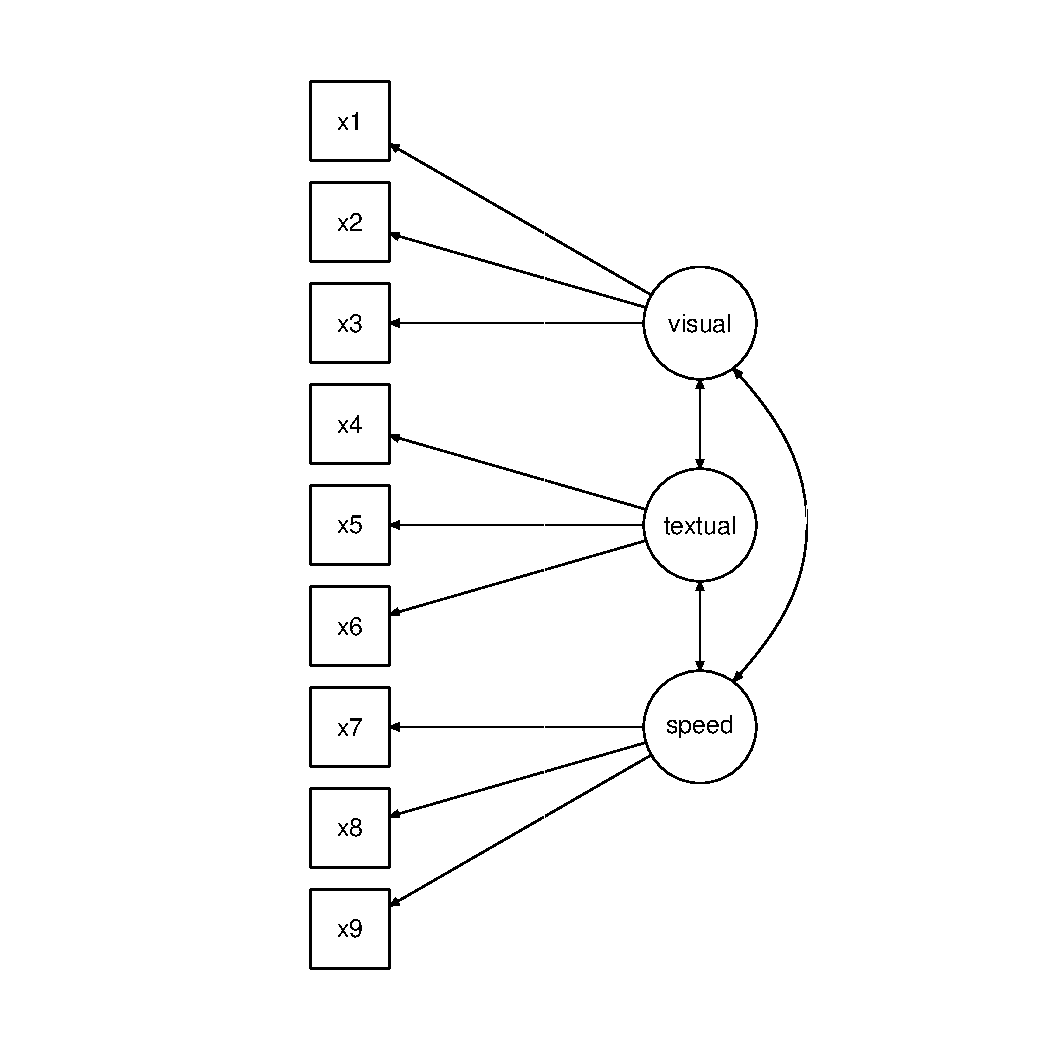
\includegraphics{figure/cfa.pdf}

The corresponding lavaan syntax for specifying this model is as follows:

\begin{verbatim}
 visual =~ x1 + x2 + x3
textual =~ x4 + x5 + x6
  speed =~ x7 + x8 + x9
\end{verbatim}

In this example, the model syntax only contains three `latent variable
definitions'. Each formula has the following format:

\begin{verbatim}
latent variable =~ indicator1 + indicator2 + indicator3
\end{verbatim}

We call these expressions \emph{latent variable definitions} because
they define how the latent variables are `manifested by' a set of
observed (or manifest) variables, often called `indicators'. Note that
the special ``\texttt{=\textasciitilde{}"} operator in the middle
consists of a sign (''\texttt{=}``) character and a tilde
(\texttt{"\textasciitilde{}"}) character next to each other. The reason
why this model syntax is so short, is that behind the scenes, the
function will take care of several things. First, by default, the factor
loading of the first indicator of a latent variable is fixed to 1,
thereby fixing the scale of the latent variable. Second, residual
variances are added automatically. And third, all exogenous latent
variables are correlated by default. This way, the model syntax can be
kept concise. On the other hand, the user remains in control, since all
this `default' behavior can be overriden and/or switched off.

We can enter the model syntax using the single quotes:

\begin{Shaded}
\begin{Highlighting}[]
\NormalTok{HS.model <-}\StringTok{ ' visual  =~ x1 + x2 + x3 }
\StringTok{              textual =~ x4 + x5 + x6}
\StringTok{              speed   =~ x7 + x8 + x9 '}
\end{Highlighting}
\end{Shaded}

We can now fit the model as follows:

\begin{Shaded}
\begin{Highlighting}[]
\NormalTok{fit <-}\StringTok{ }\KeywordTok{cfa}\NormalTok{(HS.model, }\DataTypeTok{data =} \NormalTok{HolzingerSwineford1939)}
\end{Highlighting}
\end{Shaded}

The \texttt{cfa()} function is a dedicated function for fitting
confirmatory factor analysis models. The first argument is the
user-specified model. The second argument is the dataset that contains
the observed variables. Once the model has been fitted, the
\texttt{summary()} function provides a nice summary of the fitted model:

\begin{Shaded}
\begin{Highlighting}[]
\KeywordTok{summary}\NormalTok{(fit, }\DataTypeTok{fit.measures =} \OtherTok{TRUE}\NormalTok{)}
\end{Highlighting}
\end{Shaded}

The output should look familiar to users of other SEM software. If you
find it confusing or esthetically unpleasing, please let us know, and we
will try to improve it.

\begin{verbatim}
lavaan (0.5-13) converged normally after  41 iterations

  Number of observations                           301

  Estimator                                         ML
  Minimum Function Test Statistic               85.306
  Degrees of freedom                                24
  P-value (Chi-square)                           0.000

Model test baseline model:

  Minimum Function Test Statistic              918.852
  Degrees of freedom                                36
  P-value                                        0.000

Full model versus baseline model:

  Comparative Fit Index (CFI)                    0.931
  Tucker-Lewis Index (TLI)                       0.896

Loglikelihood and Information Criteria:

  Loglikelihood user model (H0)              -3737.745
  Loglikelihood unrestricted model (H1)      -3695.092

  Number of free parameters                         21
  Akaike (AIC)                                7517.490
  Bayesian (BIC)                              7595.339
  Sample-size adjusted Bayesian (BIC)         7528.739

Root Mean Square Error of Approximation:

  RMSEA                                          0.092
  90 Percent Confidence Interval          0.071  0.114
  P-value RMSEA <= 0.05                          0.001

Standardized Root Mean Square Residual:

  SRMR                                           0.065

Parameter estimates:

  Information                                 Expected
  Standard Errors                             Standard

                   Estimate  Std.err  Z-value  P(>|z|)
Latent variables:
  visual =~
    x1                1.000
    x2                0.553    0.100    5.554    0.000
    x3                0.729    0.109    6.685    0.000
  textual =~
    x4                1.000
    x5                1.113    0.065   17.014    0.000
    x6                0.926    0.055   16.703    0.000
  speed =~
    x7                1.000
    x8                1.180    0.165    7.152    0.000
    x9                1.082    0.151    7.155    0.000

Covariances:
  visual ~~
    textual           0.408    0.074    5.552    0.000
    speed             0.262    0.056    4.660    0.000
  textual ~~
    speed             0.173    0.049    3.518    0.000

Variances:
    x1                0.549    0.114
    x2                1.134    0.102
    x3                0.844    0.091
    x4                0.371    0.048
    x5                0.446    0.058
    x6                0.356    0.043
    x7                0.799    0.081
    x8                0.488    0.074
    x9                0.566    0.071
    visual            0.809    0.145
    textual           0.979    0.112
    speed             0.384    0.086
\end{verbatim}

The output consists of three parts. The first six lines are called
\emph{the header}. The header contains the following information:

\begin{itemize}
\itemsep1pt\parskip0pt\parsep0pt
\item
  the lavaan version number
\item
  did lavaan converge normally or not, and how many iterations were
  needed
\item
  the number of observations that were effectively used in the analysis
\item
  the estimator that was used to obtain the parameter values (here:
  \texttt{ML})
\item
  the model test statistic, the degrees of freedom, and a corresponding
  p-value
\end{itemize}

The next section contains additional fit measures, and is only shown
because we use the optional argument \texttt{fit.measures = TRUE}. It
starts with the line \texttt{Model test baseline model} and ends with
the value for the \texttt{SRMR}. The last section contains the parameter
estimates. It starts with information about the standard errors (if the
information matrix is expected or observed, and if the standard errors
are standard, robust, or based on the bootstrap). Then, it tabulates all
free (and fixed) parameters that were included in the model. Typically,
first the latent variables are shown, followed by covariances and
(residual) variances. The first column (\texttt{Estimate}) contains the
(estimated or fixed) parameter value for each model parameter; the
second column (\texttt{Std.err}) contains the standard error for each
estimated parameter; the third column (\texttt{Z-value}) contains the
Wald statistic (which is simply obtained by dividing the parameter value
by its standard error), and the last column
(\texttt{P(\textgreater{}\textbar{}z\textbar{})}) contains the p-value
for testing the null hypothesis that the parameter equals zero in the
population.

To wrap up this first example, we summarize the complete code that was
needed to fit this three-factor model:

\begin{Shaded}
\begin{Highlighting}[]
\CommentTok{# load the lavaan package (only needed once per session)}
\KeywordTok{library}\NormalTok{(lavaan)}

\CommentTok{# specify the model}
\NormalTok{HS.model <-}\StringTok{ ' visual  =~ x1 + x2 + x3      }
\StringTok{              textual =~ x4 + x5 + x6}
\StringTok{              speed   =~ x7 + x8 + x9 '}

\CommentTok{# fit the model}
\NormalTok{fit <-}\StringTok{ }\KeywordTok{cfa}\NormalTok{(HS.model, }\DataTypeTok{data=}\NormalTok{HolzingerSwineford1939)}

\CommentTok{# display summary output}
\KeywordTok{summary}\NormalTok{(fit, }\DataTypeTok{fit.measures=}\OtherTok{TRUE}\NormalTok{)}
\end{Highlighting}
\end{Shaded}

Simply copying this code and pasting it in R should work. The syntax
illustrates the typical workflow in the lavaan package:

\begin{enumerate}
\def\labelenumi{\arabic{enumi}.}
\item
  Specify your model using the lavaan model syntax. In this example,
  only \emph{latent variable definitions} have been used. In the
  following examples, other formula types will be used.
\item
  Fit the model. This requires a dataset containing the observed
  variables (or alternatively the sample covariance matrix and the
  number of observations). In this example, we have used the
  \texttt{cfa()} function. Other funcions in the lavaan package are
  \texttt{sem()} and \texttt{growth()} for fitting full structural
  equation models and growth curve models respectively. All three
  functions are so-called user-friendly functions, in the sense that
  they take care of many details automatically, so we can keep the model
  syntax simple and concise. If you wish to fit non-standard models or
  if you don't like the idea that things are done for you automatically,
  you can use the lower-level function \texttt{lavaan()} instead, where
  you have full control.
\item
  Extract information from the fitted model. This can be a long verbose
  summary, or it can be a single number only (say, the RMSEA value). In
  the spirit of R, you only get what you asked for. We try to not print
  out unnecessary information that you would ignore anyway.
\end{enumerate}

\section{A second example: a structural equation model (SEM)}
In our second example, we will use the built-in
\texttt{PoliticalDemocracy} dataset. This is a dataset that has been
used by Bollen in his 1989 book on structural equation modeling (and
elsewhere). To learn more about the dataset, see its help page and the
references therein.

The figure below contains a graphical representation of the model that
we want to fit.

The corresponding lavaan syntax for specifying this model is as follows:

\begin{Shaded}
\begin{Highlighting}[]
\NormalTok{model <-}\StringTok{ '}
\StringTok{  # measurement model}
\StringTok{    ind60 =~ x1 + x2 + x3}
\StringTok{    dem60 =~ y1 + y2 + y3 + y4}
\StringTok{    dem65 =~ y5 + y6 + y7 + y8}
\StringTok{  # regressions}
\StringTok{    dem60 ~ ind60}
\StringTok{    dem65 ~ ind60 + dem60}
\StringTok{  # residual correlations}
\StringTok{    y1 ~~ y5}
\StringTok{    y2 ~~ y4 + y6}
\StringTok{    y3 ~~ y7}
\StringTok{    y4 ~~ y8}
\StringTok{    y6 ~~ y8}
\StringTok{'}
\end{Highlighting}
\end{Shaded}

In this example, we use three different formula types: latent variabele
definitions (using the \texttt{=\textasciitilde{}} operator), regression
formulas (using the \texttt{\textasciitilde{}} operator), and
(co)variance formulas (using the
\texttt{\textasciitilde{}\textasciitilde{}} operator). The regression
formulas are similar to ordinary formulas in R. The (co)variance
formulas typically have the following form:

\begin{verbatim}
variable ~~ variable
\end{verbatim}

The variables can be either observed or latent variables. If the two
variable names are the same, the expression refers to the variance (or
residual variance) of that variable. If the two variable names are
different, the expression refers to the (residual) covariance among
these two variables. The lavaan package automatically makes the
distinction between variances and residual variances.

In our example, the expression
\texttt{y1 \textasciitilde{}\textasciitilde{} y5} allows the residual
variances of the two observed variables to be correlated. This is
sometimes done if it is believed that the two variables have something
in common that is not captured by the latent variables. In this case,
the two variables refer to identical scores, but measured in two
different years (1960 and 1965, respectively). Note that the two
expressions \texttt{y2 \textasciitilde{}\textasciitilde{} y4} and
\texttt{y2 \textasciitilde{}\textasciitilde{} y6}, can be combined into
the expression \texttt{y2 \textasciitilde{}\textasciitilde{}~y4 + y6}.
This is just a shorthand notation.

We enter the model syntax as follows:

\begin{Shaded}
\begin{Highlighting}[]
\NormalTok{model <-}\StringTok{ '}
\StringTok{  # measurement model}
\StringTok{    ind60 =~ x1 + x2 + x3}
\StringTok{    dem60 =~ y1 + y2 + y3 + y4}
\StringTok{    dem65 =~ y5 + y6 + y7 + y8}
\StringTok{  # regressions}
\StringTok{    dem60 ~ ind60}
\StringTok{    dem65 ~ ind60 + dem60}
\StringTok{  # residual correlations}
\StringTok{    y1 ~~ y5}
\StringTok{    y2 ~~ y4 + y6}
\StringTok{    y3 ~~ y7}
\StringTok{    y4 ~~ y8}
\StringTok{    y6 ~~ y8}
\StringTok{'}
\end{Highlighting}
\end{Shaded}

To fit the model and see the results we can type:

\begin{Shaded}
\begin{Highlighting}[]
\NormalTok{fit <-}\StringTok{ }\KeywordTok{sem}\NormalTok{(model, }\DataTypeTok{data =} \NormalTok{PoliticalDemocracy)}
\KeywordTok{summary}\NormalTok{(fit, }\DataTypeTok{standardized =} \OtherTok{TRUE}\NormalTok{)}
\end{Highlighting}
\end{Shaded}

\begin{verbatim}
lavaan (0.5-13) converged normally after  68 iterations

  Number of observations                            75

  Estimator                                         ML
  Minimum Function Test Statistic               38.125
  Degrees of freedom                                35
  P-value (Chi-square)                           0.329

Parameter estimates:

  Information                                 Expected
  Standard Errors                             Standard

                   Estimate  Std.err  Z-value  P(>|z|)   Std.lv  Std.all
Latent variables:
  ind60 =~
    x1                1.000                               0.670    0.920
    x2                2.180    0.139   15.742    0.000    1.460    0.973
    x3                1.819    0.152   11.967    0.000    1.218    0.872
  dem60 =~
    y1                1.000                               2.223    0.850
    y2                1.257    0.182    6.889    0.000    2.794    0.717
    y3                1.058    0.151    6.987    0.000    2.351    0.722
    y4                1.265    0.145    8.722    0.000    2.812    0.846
  dem65 =~
    y5                1.000                               2.103    0.808
    y6                1.186    0.169    7.024    0.000    2.493    0.746
    y7                1.280    0.160    8.002    0.000    2.691    0.824
    y8                1.266    0.158    8.007    0.000    2.662    0.828

Regressions:
  dem60 ~
    ind60             1.483    0.399    3.715    0.000    0.447    0.447
  dem65 ~
    ind60             0.572    0.221    2.586    0.010    0.182    0.182
    dem60             0.837    0.098    8.514    0.000    0.885    0.885

Covariances:
  y1 ~~
    y5                0.624    0.358    1.741    0.082    0.624    0.296
  y2 ~~
    y4                1.313    0.702    1.871    0.061    1.313    0.273
    y6                2.153    0.734    2.934    0.003    2.153    0.356
  y3 ~~
    y7                0.795    0.608    1.308    0.191    0.795    0.191
  y4 ~~
    y8                0.348    0.442    0.787    0.431    0.348    0.109
  y6 ~~
    y8                1.356    0.568    2.386    0.017    1.356    0.338

Variances:
    x1                0.082    0.019                      0.082    0.154
    x2                0.120    0.070                      0.120    0.053
    x3                0.467    0.090                      0.467    0.239
    y1                1.891    0.444                      1.891    0.277
    y2                7.373    1.374                      7.373    0.486
    y3                5.067    0.952                      5.067    0.478
    y4                3.148    0.739                      3.148    0.285
    y5                2.351    0.480                      2.351    0.347
    y6                4.954    0.914                      4.954    0.443
    y7                3.431    0.713                      3.431    0.322
    y8                3.254    0.695                      3.254    0.315
    ind60             0.448    0.087                      1.000    1.000
    dem60             3.956    0.921                      0.800    0.800
    dem65             0.172    0.215                      0.039    0.039
\end{verbatim}

The function \texttt{sem()} is very similar to the function
\texttt{cfa()}. In fact, the two functions are currently almost
identical, but this may change in the future. In the \texttt{summary()}
function, we omitted the \texttt{fit.measures=TRUE} argument. Therefore,
you only get the basic chi-square test statistic. The argument
\texttt{standardized=TRUE} augments the output with standardized
parameter values. Two extra columns of standardized parameter values are
printed. In the first column (labeled \texttt{Std.lv}), only the latent
variables are standardized. In the second column (labeled
\texttt{Std.all}), both latent and observed variables are standardized.
The latter is often called the `completely standardized solution'.

The complete code to specify and fit this model is printed again below:

\begin{Shaded}
\begin{Highlighting}[]
\KeywordTok{library}\NormalTok{(lavaan) }\CommentTok{# only needed once per session}
\NormalTok{model <-}\StringTok{ '}
\StringTok{  # measurement model}
\StringTok{    ind60 =~ x1 + x2 + x3}
\StringTok{    dem60 =~ y1 + y2 + y3 + y4}
\StringTok{    dem65 =~ y5 + y6 + y7 + y8}
\StringTok{  # regressions}
\StringTok{    dem60 ~ ind60}
\StringTok{    dem65 ~ ind60 + dem60}
\StringTok{  # residual correlations}
\StringTok{    y1 ~~ y5}
\StringTok{    y2 ~~ y4 + y6}
\StringTok{    y3 ~~ y7}
\StringTok{    y4 ~~ y8}
\StringTok{    y6 ~~ y8}
\StringTok{'}
\NormalTok{fit <-}\StringTok{ }\KeywordTok{sem}\NormalTok{(model, }\DataTypeTok{data=}\NormalTok{PoliticalDemocracy)}
\KeywordTok{summary}\NormalTok{(fit, }\DataTypeTok{standardized=}\OtherTok{TRUE}\NormalTok{)}
\end{Highlighting}
\end{Shaded}


\section{More about the syntax}
\paragraph{Fixing parameters}

Consider a simple one-factor model with 4 indicators. By default, lavaan
will always fix the factor loading of the first indicator to 1. The
other three factor loadings are free, and their values are estimated by
the model. But suppose that you have good reasons the fix all the factor
loadings to 1. The syntax below illustrates how this can be done:

\begin{verbatim}
f =~ y1 + 1*y2 + 1*y3 + 1*y4
\end{verbatim}

In general, to fix a parameter in a lavaan formula, you need to
pre-multiply the corresponding variable in the formula by a numerical
value. This is called the pre-multiplication mechanism and will be used
for many purposes. As another example, consider again the three-factor
Holzinger and Swineford CFA model. Recall that, by default, all
exogenous latent variables in a CFA model are correlated. But if you
wish to fix the correlation (or covariance) between a pair of latent
variables to zero, you need to explicity add a covariance-formula for
this pair, and fix the parameter to zero. In the syntax below, we allow
the covariance between the latent variables \texttt{visual} and
\texttt{textual} to be free, but the two other covariances are fixed to
zero. In addition, we fix the variance of the factor \texttt{speed} to
unity. Therefore, there is no need anymore to set the factor loading of
its first indicator (\texttt{x7}) equal to one. To force this factor
loading to be free, we pre-multiply it with \texttt{NA}, as a hint to
lavaan that the value of this parameter is still unknown.

\begin{verbatim}
# three-factor model
   visual =~ x1 + x2 + x3
  textual =~ x4 + x5 + x6
  speed   =~ NA*x7 + x8 + x9
# orthogonal factors
   visual ~~ 0*speed
  textual ~~ 0*speed
# fix variance of speed factor
    speed ~~ 1*speed
\end{verbatim}

If you need to constrain all covariances of the latent variables in a
CFA model to be orthogonal, there is a shortcut. You can omit the
covariance formulas in the model syntax and simply add an argument
\texttt{orthogonal=TRUE} to the function call:

\begin{Shaded}
\begin{Highlighting}[]
\NormalTok{HS.model <-}\StringTok{ '  visual =~ x1 + x2 + x3}
\StringTok{              textual =~ x4 + x5 + x6}
\StringTok{              speed   =~ x7 + x8 + x9 '}

\NormalTok{fit.HS.ortho <-}\StringTok{ }\KeywordTok{cfa}\NormalTok{(HS.model, }
                    \DataTypeTok{data =} \NormalTok{HolzingerSwineford1939, }
                    \DataTypeTok{orthogonal =} \OtherTok{TRUE}\NormalTok{)}
\end{Highlighting}
\end{Shaded}

Similarly, if you want to fix the variances of \emph{all} the latent
variables in a CFA model to unity, there is again a shortcut. Simply add
the argument \texttt{std.lv=TRUE} to the function call:

\begin{Shaded}
\begin{Highlighting}[]
\NormalTok{HS.model <-}\StringTok{ ' visual  =~ x1 + x2 + x3}
\StringTok{              textual =~ x4 + x5 + x6}
\StringTok{              speed   =~ x7 + x8 + x9 '}
\NormalTok{fit <-}\StringTok{ }\KeywordTok{cfa}\NormalTok{(HS.model, }
           \DataTypeTok{data =} \NormalTok{HolzingerSwineford1939, }
           \DataTypeTok{std.lv =} \OtherTok{TRUE}\NormalTok{)}
\end{Highlighting}
\end{Shaded}

If the argument \texttt{std.lv=TRUE} is used, the factor loadings of the
first indicator of each latent variable will no longer be fixed to 1.

\paragraph{Starting Values}

The lavaan package automatically generates starting values for all free
parameters. Normally, this works fine. But if you must provide your own
starting values, you are free to do so. The way it works is based on the
pre-multiplication mechanism that we discussed before. But the numeric
constant is now the argument of a special function \texttt{start()}. An
example will make this clear:

\begin{verbatim}
 visual =~ x1 + start(0.8)*x2 + start(1.2)*x3
textual =~ x4 + start(0.5)*x5 + start(1.0)*x6
speed   =~ x7 + start(0.7)*x8 + start(1.8)*x9
\end{verbatim}

\paragraph{Parameter labels}

A nice property of the lavaan package is that all free parameters are
automatically named according to a simple set of rules. This is
convenient, for example, if equality constraints are needed (see the
next subsection). To see how the naming mechanism works, we will use the
model that we used for the Politcal Democracy data.

\begin{Shaded}
\begin{Highlighting}[]
\NormalTok{model <-}\StringTok{ '}
\StringTok{  # latent variable definitions}
\StringTok{    ind60 =~ x1 + x2 + x3}
\StringTok{    dem60 =~ y1 + y2 + y3 + y4}
\StringTok{    dem65 =~ y5 + y6 + y7 + y8}
\StringTok{  # regressions}
\StringTok{    dem60 ~ ind60}
\StringTok{    dem65 ~ ind60 + dem60}
\StringTok{  # residual (co)variances}
\StringTok{    y1 ~~ y5}
\StringTok{    y2 ~~ y4 + y6}
\StringTok{    y3 ~~ y7}
\StringTok{    y4 ~~ y8}
\StringTok{    y6 ~~ y8}
\StringTok{'}
\NormalTok{fit <-}\StringTok{ }\KeywordTok{sem}\NormalTok{(model, }
           \DataTypeTok{data =} \NormalTok{PoliticalDemocracy)}
\KeywordTok{coef}\NormalTok{(fit)}
\end{Highlighting}
\end{Shaded}

\begin{verbatim}
   ind60=~x2    ind60=~x3    dem60=~y2    dem60=~y3    dem60=~y4 
       2.180        1.819        1.257        1.058        1.265 
   dem65=~y6    dem65=~y7    dem65=~y8  dem60~ind60  dem65~ind60 
       1.186        1.280        1.266        1.483        0.572 
 dem65~dem60       y1~~y5       y2~~y4       y2~~y6       y3~~y7 
       0.837        0.624        1.313        2.153        0.795 
      y4~~y8       y6~~y8       x1~~x1       x2~~x2       x3~~x3 
       0.348        1.356        0.082        0.120        0.467 
      y1~~y1       y2~~y2       y3~~y3       y4~~y4       y5~~y5 
       1.891        7.373        5.067        3.148        2.351 
      y6~~y6       y7~~y7       y8~~y8 ind60~~ind60 dem60~~dem60 
       4.954        3.431        3.254        0.448        3.956 
dem65~~dem65 
       0.172 
\end{verbatim}

The function \texttt{coef()} extracts the estimated values of the free
parameters in the model, together with their names. Each name consists
of three parts and reflects the part of the formula where the parameter
was involved. The first part is the variable name that appears on the
left-hand side of the formula. The middle part is the operator type of
the formula, and the third part is the variable in the right-hand side
of the formula that corresponds with the parameter.

Often, it is convenient to choose your own labels for specific
parameters. The way this works is similar to fixing a parameter. But
instead of pre-multiplying with a numerical constant, we use a character
string (the label) instead. In the example below, we `label' the factor
loading of the \texttt{x3} indicator with the label \texttt{myLabel}:

\begin{Shaded}
\begin{Highlighting}[]
\NormalTok{model <-}\StringTok{ '}
\StringTok{  # latent variable definitions}
\StringTok{    ind60 =~ x1 + x2 + myLabel*x3}
\StringTok{    dem60 =~ y1 + y2 + y3 + y4}
\StringTok{    dem65 =~ y5 + y6 + y7 + y8}
\StringTok{  # regressions}
\StringTok{    dem60 ~ ind60}
\StringTok{    dem65 ~ ind60 + dem60}
\StringTok{  # residual (co)variances}
\StringTok{    y1 ~~ y5}
\StringTok{    y2 ~~ y4 + y6}
\StringTok{    y3 ~~ y7}
\StringTok{    y4 ~~ y8}
\StringTok{    y6 ~~ y8}
\StringTok{'}
\end{Highlighting}
\end{Shaded}

It is important that labels start with a letter (a-zA-Z), and certainly
not with a digit. For example `13bis' is not a valid label, and will
confuse the lavaan syntax parser. Note: before version 0.4-8, it was
necessary to use the modifier \texttt{label()} to specify a custom
label. Although it is still supported, it is not recommended anymore.
The only reason why it should be used in new syntax is if the label
contains an operator like ``\texttt{\textasciitilde{}}'' or
``\texttt{=\textasciitilde{}}''.

\paragraph{Modifiers}

We have seen the use of the pre-multiplication mechanism (using the
\texttt{*} operator) a number of times: to fix a parameter, to provide a
starting value, and to label a parameter. We refer to these operations
as \emph{modifiers}, because they modify some properties of certain
model parameters. More modifiers will be introduced later.

Each term on the right hand side in a formula can have one modifier
only. If you must specify more modifiers for the same parameter, you
need to list the term multiple times in the same formula. For example:

\begin{verbatim}
f =~ y1 + y2 + myLabel*y3 + start(0.5)*y3 + y4
\end{verbatim}

The indicator \texttt{y3} was listed twice, each time with a different
modifier. The parser will accumulate all the different modifiers, but
still treat \texttt{y3} as a single indicator.

\paragraph{Simple equality constraints}

In some applications, it is useful to impose equality constraints on one
or more otherwise free parameters. Consider again the three-factor H\&S
CFA model. Suppose a user has a priori reasons to believe that the
factor loadings of the \texttt{x2} and \texttt{x3} indicators are equal
to each other. Instead of estimating two free parameters, lavaan should
only estimate a single free parameter, and use that value for both
factor loadings. The main mechanism to specify this type of (simple)
equality constraints is by using labels: if two parameters have the same
label, they will be considered to be the same, and only one value will
be computed for them. This is illustrated in the following syntax:

\begin{verbatim}
 visual =~ x1 + v2*x2 + v2*x3
textual =~ x4 + x5 + x6
speed   =~ x7 + x8 + x9
\end{verbatim}

Remember: all parameters having the same label will be constrained to be
equal.

An alternative approach is to use the \texttt{equal()} modifier. This is
useful if no custom label has been specified, and one needs to refer to
the automatically generated label. For example:

\begin{verbatim}
 visual =~ x1 + x2 + equal("visual=~x2")*x3
textual =~ x4 + x5 + x6
speed   =~ x7 + x8 + x9
\end{verbatim}

\paragraph{Nonlinear equality and inequality constraints}

Consider the following regression:

\begin{verbatim}
y ~ b1*x1 + b2*x2 + b3*x3
\end{verbatim}

where we have explicitly labeled the regression coefficients as
\texttt{b1}, \texttt{b2} and \texttt{b3}. We create a toy dataset
containing these four variables and fit the regression model:

\begin{Shaded}
\begin{Highlighting}[]
\KeywordTok{set.seed}\NormalTok{(}\DecValTok{1234}\NormalTok{)}
\NormalTok{Data <-}\StringTok{ }\KeywordTok{data.frame}\NormalTok{(}\DataTypeTok{y =} \KeywordTok{rnorm}\NormalTok{(}\DecValTok{100}\NormalTok{), }
                   \DataTypeTok{x1 =} \KeywordTok{rnorm}\NormalTok{(}\DecValTok{100}\NormalTok{), }
                   \DataTypeTok{x2 =} \KeywordTok{rnorm}\NormalTok{(}\DecValTok{100}\NormalTok{),}
                   \DataTypeTok{x3 =} \KeywordTok{rnorm}\NormalTok{(}\DecValTok{100}\NormalTok{))}
\NormalTok{model <-}\StringTok{ ' y ~ b1*x1 + b2*x2 + b3*x3 '}
\NormalTok{fit <-}\StringTok{ }\KeywordTok{sem}\NormalTok{(model, }\DataTypeTok{data=}\NormalTok{Data)}
\KeywordTok{coef}\NormalTok{(fit)}
\end{Highlighting}
\end{Shaded}

\begin{verbatim}
    b1     b2     b3   y~~y 
-0.052  0.084  0.139  0.970 
\end{verbatim}

Suppose that we need to impose the following two (nonlinear) constraints
on $b_1$: $b_1 = (b_2+b_3)^2$ and $b_1 \geq \exp(b_2 + b_3)$. The first
constraint is an equality constraint. The second is an inequality
constraint. To specify these constraints, you can use the following
syntax:

\begin{Shaded}
\begin{Highlighting}[]
\NormalTok{model.constr <-}\StringTok{ ' # model with labeled parameters}
\StringTok{                    y ~ b1*x1 + b2*x2 + b3*x3}
\StringTok{                  # constraints}
\StringTok{                    b1 == (b2 + b3)^2}
\StringTok{                    b1 > exp(b2 + b3) '}
\end{Highlighting}
\end{Shaded}

To see the effect of the constraints, we refit the model:

\begin{Shaded}
\begin{Highlighting}[]
\NormalTok{model.constr <-}\StringTok{ ' # model with labeled parameters}
\StringTok{                    y ~ b1*x1 + b2*x2 + b3*x3}
\StringTok{                  # constraints}
\StringTok{                    b1 == (b2 + b3)^2}
\StringTok{                    b1 > exp(b2 + b3) '}
\NormalTok{fit <-}\StringTok{ }\KeywordTok{sem}\NormalTok{(model.constr, }\DataTypeTok{data=}\NormalTok{Data)}
\KeywordTok{coef}\NormalTok{(fit)}
\end{Highlighting}
\end{Shaded}

\begin{verbatim}
    b1     b2     b3   y~~y 
 0.495 -0.405 -0.299  1.610 
\end{verbatim}

The reader can verify that the constraints are indeed respected. The
equality constraint holds exactly. The inequality constraint has
resulted in an equality between the left-hand side ($b_1$) and the
right-hand side ($\exp(b_2 + b_3)$).

\section{Bringing in the means}
By and large, structural equation models are used to model the
covariance matrix of the observed variables in a dataset. But in some
applications, it is useful to bring in the means of the observed
variables too. One way to do this is to explicitly refer to intercepts
in the lavaan syntax. This can be done by including `intercept formulas'
in the model syntax. An intercept formula has the following form:

\begin{verbatim}
variable ~ 1
\end{verbatim}

The left part of the expression contains the name of the observed or
latent variable. The right part contains the number \texttt{1},
representing the intercept. For example, in the three-factor H\&S CFA
model, we can add the intercepts of the observed variables as follows:

\begin{verbatim}
# three-factor model
   visual =~ x1 + x2 + x3
  textual =~ x4 + x5 + x6
  speed   =~ x7 + x8 + x9
# intercepts
  x1 ~ 1
  x2 ~ 1
  x3 ~ 1
  x4 ~ 1
  x5 ~ 1
  x6 ~ 1
  x7 ~ 1
  x8 ~ 1
  x9 ~ 1
\end{verbatim}

However, it is more convenient to omit the intercept formulas in the
model syntax (unless you want to fix their values), and to add the
argument \texttt{meanstructure = TRUE} in the fitting function. For
example, we can refit the three-factor H\&S CFA model as follows:

\begin{Shaded}
\begin{Highlighting}[]
\NormalTok{fit <-}\StringTok{ }\KeywordTok{cfa}\NormalTok{(HS.model, }
           \DataTypeTok{data =} \NormalTok{HolzingerSwineford1939, }
           \DataTypeTok{meanstructure =} \OtherTok{TRUE}\NormalTok{)}
\KeywordTok{summary}\NormalTok{(fit)}
\end{Highlighting}
\end{Shaded}

\begin{verbatim}
lavaan (0.5-13) converged normally after  41 iterations

  Number of observations                           301

  Estimator                                         ML
  Minimum Function Test Statistic               85.306
  Degrees of freedom                                24
  P-value (Chi-square)                           0.000

Parameter estimates:

  Information                                 Expected
  Standard Errors                             Standard

                   Estimate  Std.err  Z-value  P(>|z|)
Latent variables:
  visual =~
    x1                1.000
    x2                0.553    0.100    5.554    0.000
    x3                0.729    0.109    6.685    0.000
  textual =~
    x4                1.000
    x5                1.113    0.065   17.014    0.000
    x6                0.926    0.055   16.703    0.000
  speed =~
    x7                1.000
    x8                1.180    0.165    7.152    0.000
    x9                1.082    0.151    7.155    0.000

Covariances:
  visual ~~
    textual           0.408    0.074    5.552    0.000
    speed             0.262    0.056    4.660    0.000
  textual ~~
    speed             0.173    0.049    3.518    0.000

Intercepts:
    x1                4.936    0.067   73.473    0.000
    x2                6.088    0.068   89.855    0.000
    x3                2.250    0.065   34.579    0.000
    x4                3.061    0.067   45.694    0.000
    x5                4.341    0.074   58.452    0.000
    x6                2.186    0.063   34.667    0.000
    x7                4.186    0.063   66.766    0.000
    x8                5.527    0.058   94.854    0.000
    x9                5.374    0.058   92.546    0.000
    visual            0.000
    textual           0.000
    speed             0.000

Variances:
    x1                0.549    0.114
    x2                1.134    0.102
    x3                0.844    0.091
    x4                0.371    0.048
    x5                0.446    0.058
    x6                0.356    0.043
    x7                0.799    0.081
    x8                0.488    0.074
    x9                0.566    0.071
    visual            0.809    0.145
    textual           0.979    0.112
    speed             0.384    0.086
\end{verbatim}

As you can see in the output, the model includes intercept parameters
for both the observed and latent variables. By default, the
\texttt{cfa()} and \texttt{sem()} functions fix the latent variable
intercepts (which in this case correspond to the latent \emph{means}) to
zero. Otherwise, the model would not be estimable. Note that the
chi-square statistic and the number of degrees of freedom is the same as
in the original model (without a mean structure). The reason is that we
brought in some new data (a mean value for each of the 9 observed
variables), but we also added 9 additional parameters to the model (an
intercept for each of the 9 observed variables). The end result is an
identical fit. In practice, the only reason why a user would add
intercept-formulas in the model syntax, is because some constraints must
be specified on them. For example, suppose that we wish to fix the
intercepts of the variables \texttt{x1}, \texttt{x2}, \texttt{x3} and
\texttt{x4} to, say, 0.5. We would write the model syntax as follows:

\begin{verbatim}
# three-factor model
   visual =~ x1 + x2 + x3
  textual =~ x4 + x5 + x6
  speed   =~ x7 + x8 + x9
# intercepts with fixed values
  x1 + x2 + x3 + x4 ~ 0.5*1
\end{verbatim}

where we have used the left-hand side of the formula to `repeat' the
right-hand side for each element of the left-hand side.

\section{Multiple groups}
The lavaan package has full support for multiple groups. To request a
multiple group analysis, you need to add the name of the group variable
in your dataset to the argument \texttt{group} in the fitting function.
By default, the same model is fitted in all groups. In the following
example, we fit the H\&S CFA model for the two schools (Pasteur and
Grant-White).

\begin{Shaded}
\begin{Highlighting}[]
\NormalTok{HS.model <-}\StringTok{ '  visual =~ x1 + x2 + x3}
\StringTok{              textual =~ x4 + x5 + x6}
\StringTok{              speed   =~ x7 + x8 + x9 '}
\NormalTok{fit <-}\StringTok{ }\KeywordTok{cfa}\NormalTok{(HS.model, }
           \DataTypeTok{data =} \NormalTok{HolzingerSwineford1939, }
           \DataTypeTok{group =} \StringTok{"school"}\NormalTok{)}
\KeywordTok{summary}\NormalTok{(fit)}
\end{Highlighting}
\end{Shaded}

\begin{verbatim}
lavaan (0.5-13) converged normally after  63 iterations

  Number of observations per group         
  Pasteur                                          156
  Grant-White                                      145

  Estimator                                         ML
  Minimum Function Test Statistic              115.851
  Degrees of freedom                                48
  P-value (Chi-square)                           0.000

Chi-square for each group:

  Pasteur                                       64.309
  Grant-White                                   51.542

Parameter estimates:

  Information                                 Expected
  Standard Errors                             Standard

Group 1 [Pasteur]:

                   Estimate  Std.err  Z-value  P(>|z|)
Latent variables:
  visual =~
    x1                1.000
    x2                0.394    0.122    3.220    0.001
    x3                0.570    0.140    4.076    0.000
  textual =~
    x4                1.000
    x5                1.183    0.102   11.613    0.000
    x6                0.875    0.077   11.421    0.000
  speed =~
    x7                1.000
    x8                1.125    0.277    4.057    0.000
    x9                0.922    0.225    4.104    0.000

Covariances:
  visual ~~
    textual           0.479    0.106    4.531    0.000
    speed             0.185    0.077    2.397    0.017
  textual ~~
    speed             0.182    0.069    2.628    0.009

Intercepts:
    x1                4.941    0.095   52.249    0.000
    x2                5.984    0.098   60.949    0.000
    x3                2.487    0.093   26.778    0.000
    x4                2.823    0.092   30.689    0.000
    x5                3.995    0.105   38.183    0.000
    x6                1.922    0.079   24.321    0.000
    x7                4.432    0.087   51.181    0.000
    x8                5.563    0.078   71.214    0.000
    x9                5.418    0.079   68.440    0.000
    visual            0.000
    textual           0.000
    speed             0.000

Variances:
    x1                0.298    0.232
    x2                1.334    0.158
    x3                0.989    0.136
    x4                0.425    0.069
    x5                0.456    0.086
    x6                0.290    0.050
    x7                0.820    0.125
    x8                0.510    0.116
    x9                0.680    0.104
    visual            1.097    0.276
    textual           0.894    0.150
    speed             0.350    0.126



Group 2 [Grant-White]:

                   Estimate  Std.err  Z-value  P(>|z|)
Latent variables:
  visual =~
    x1                1.000
    x2                0.736    0.155    4.760    0.000
    x3                0.925    0.166    5.583    0.000
  textual =~
    x4                1.000
    x5                0.990    0.087   11.418    0.000
    x6                0.963    0.085   11.377    0.000
  speed =~
    x7                1.000
    x8                1.226    0.187    6.569    0.000
    x9                1.058    0.165    6.429    0.000

Covariances:
  visual ~~
    textual           0.408    0.098    4.153    0.000
    speed             0.276    0.076    3.639    0.000
  textual ~~
    speed             0.222    0.073    3.022    0.003

Intercepts:
    x1                4.930    0.095   51.696    0.000
    x2                6.200    0.092   67.416    0.000
    x3                1.996    0.086   23.195    0.000
    x4                3.317    0.093   35.625    0.000
    x5                4.712    0.096   48.986    0.000
    x6                2.469    0.094   26.277    0.000
    x7                3.921    0.086   45.819    0.000
    x8                5.488    0.087   63.174    0.000
    x9                5.327    0.085   62.571    0.000
    visual            0.000
    textual           0.000
    speed             0.000

Variances:
    x1                0.715    0.126
    x2                0.899    0.123
    x3                0.557    0.103
    x4                0.315    0.065
    x5                0.419    0.072
    x6                0.406    0.069
    x7                0.600    0.091
    x8                0.401    0.094
    x9                0.535    0.089
    visual            0.604    0.160
    textual           0.942    0.152
    speed             0.461    0.118
\end{verbatim}

If you want to fix parameters, or provide starting values, you can use
the same pre-multiplication techniques, but the single argument is now
replaced by a \emph{vector} of arguments, one for each group. If you use
a single element instead of a vector, that element will be applied for
all groups (note: this is NOT true for labels, since this would imply
equality constraints). For example:

\begin{Shaded}
\begin{Highlighting}[]
\NormalTok{HS.model <-}\StringTok{ '  visual =~ x1 + 0.5*x2 + c(0.6, 0.8)*x3}
\StringTok{              textual =~ x4 + start(c(1.2, 0.6))*x5 + a*x6}
\StringTok{              speed   =~ x7 + x8 + x9 '}
\end{Highlighting}
\end{Shaded}

In the definition of the latent factor \texttt{visual}, we have fixed
the factor loading of the indicator \texttt{x3} to the value `0.6' in
the first group, and to the value `0.8' in the second group, while the
factor loading of the indicator is fixed to the value `0.5' in both
groups. In the definition of the \texttt{textual} factor, two different
starting values are provided for the \texttt{x5} indicator; one for each
group. In addition, we have labeled the factor loading of the
\texttt{x6} indicator as `a', but this label is only given to the
parameter of the first group. If you want to provide labels to each of
the two groups, you can write something like \texttt{c(a1,a2)*x6}. Be
careful: if you write \texttt{c(a,a)*x6}, both parameters (in the first
and second group) will get the same label, and hence they will be
treated as a single parameter. To verify the effects of these modifiers,
we refit the model:

\begin{Shaded}
\begin{Highlighting}[]
\NormalTok{fit <-}\StringTok{ }\KeywordTok{cfa}\NormalTok{(HS.model, }
           \DataTypeTok{data =} \NormalTok{HolzingerSwineford1939, }
           \DataTypeTok{group =} \StringTok{"school"}\NormalTok{)}
 \KeywordTok{summary}\NormalTok{(fit)}
\end{Highlighting}
\end{Shaded}

\begin{verbatim}
lavaan (0.5-13) converged normally after  58 iterations

  Number of observations per group         
  Pasteur                                          156
  Grant-White                                      145

  Estimator                                         ML
  Minimum Function Test Statistic              118.976
  Degrees of freedom                                52
  P-value (Chi-square)                           0.000

Chi-square for each group:

  Pasteur                                       64.901
  Grant-White                                   54.075

Parameter estimates:

  Information                                 Expected
  Standard Errors                             Standard

Group 1 [Pasteur]:

                   Estimate  Std.err  Z-value  P(>|z|)
Latent variables:
  visual =~
    x1                1.000
    x2                0.500
    x3                0.600
  textual =~
    x4                1.000
    x5                1.185    0.102   11.598    0.000
    x6        (a)     0.876    0.077   11.409    0.000
  speed =~
    x7                1.000
    x8                1.129    0.279    4.055    0.000
    x9                0.931    0.227    4.103    0.000

Covariances:
  visual ~~
    textual           0.460    0.103    4.479    0.000
    speed             0.182    0.076    2.408    0.016
  textual ~~
    speed             0.181    0.069    2.625    0.009

Intercepts:
    x1                4.941    0.094   52.379    0.000
    x2                5.984    0.100   59.945    0.000
    x3                2.487    0.092   26.983    0.000
    x4                2.823    0.092   30.689    0.000
    x5                3.995    0.105   38.183    0.000
    x6                1.922    0.079   24.321    0.000
    x7                4.432    0.087   51.181    0.000
    x8                5.563    0.078   71.214    0.000
    x9                5.418    0.079   68.440    0.000
    visual            0.000
    textual           0.000
    speed             0.000

Variances:
    x1                0.388    0.129
    x2                1.304    0.155
    x3                0.965    0.120
    x4                0.427    0.069
    x5                0.454    0.086
    x6                0.289    0.050
    x7                0.824    0.124
    x8                0.510    0.116
    x9                0.677    0.105
    visual            1.001    0.172
    textual           0.892    0.150
    speed             0.346    0.125



Group 2 [Grant-White]:

                   Estimate  Std.err  Z-value  P(>|z|)
Latent variables:
  visual =~
    x1                1.000
    x2                0.500
    x3                0.800
  textual =~
    x4                1.000
    x5                0.990    0.087   11.425    0.000
    x6                0.963    0.085   11.374    0.000
  speed =~
    x7                1.000
    x8                1.228    0.188    6.539    0.000
    x9                1.081    0.168    6.417    0.000

Covariances:
  visual ~~
    textual           0.454    0.099    4.585    0.000
    speed             0.315    0.079    4.004    0.000
  textual ~~
    speed             0.222    0.073    3.049    0.002

Intercepts:
    x1                4.930    0.097   50.688    0.000
    x2                6.200    0.089   69.616    0.000
    x3                1.996    0.086   23.223    0.000
    x4                3.317    0.093   35.625    0.000
    x5                4.712    0.096   48.986    0.000
    x6                2.469    0.094   26.277    0.000
    x7                3.921    0.086   45.819    0.000
    x8                5.488    0.087   63.174    0.000
    x9                5.327    0.085   62.571    0.000
    visual            0.000
    textual           0.000
    speed             0.000

Variances:
    x1                0.637    0.115
    x2                0.966    0.120
    x3                0.601    0.091
    x4                0.316    0.065
    x5                0.418    0.072
    x6                0.407    0.069
    x7                0.609    0.091
    x8                0.411    0.094
    x9                0.522    0.089
    visual            0.735    0.132
    textual           0.942    0.152
    speed             0.453    0.117
\end{verbatim}

\paragraph{Constraining a single parameter to be equal across groups}

If you want to constrain one or more parameters to be equal across
groups, you need to give them the same label. For example, to constrain
the factor loading of the indicator \texttt{x3} to be equal across (two)
groups, you can write:

\begin{Shaded}
\begin{Highlighting}[]
\NormalTok{HS.model <-}\StringTok{ '  visual =~ x1 + x2 + c(v3,v3)*x3}
\StringTok{              textual =~ x4 + x5 + x6}
\StringTok{              speed   =~ x7 + x8 + x9 '}
\end{Highlighting}
\end{Shaded}

Again, identical labels imply identical parameters, both within and
across groups.

\paragraph{Constraining groups of parameters to be equal across groups}

Although providing identical labels is a very flexible method to specify
equality constraints for a few parameters, there is a more convenient
way to impose equality constraints on a whole set of parameters (for
example: all factor loadings, or all intercepts). We call these type of
constraints \emph{group equality constraints} and they can be specified
by the argument \texttt{group.equal} in the fitting function. For
example, to constrain (all) the factor loadings to be equal across
groups, you can proceed as follows:

\begin{Shaded}
\begin{Highlighting}[]
\NormalTok{HS.model <-}\StringTok{ '  visual =~ x1 + x2 + x3}
\StringTok{              textual =~ x4 + x5 + x6}
\StringTok{              speed   =~ x7 + x8 + x9 '}
\NormalTok{fit <-}\StringTok{ }\KeywordTok{cfa}\NormalTok{(HS.model, }
           \DataTypeTok{data =} \NormalTok{HolzingerSwineford1939, }
           \DataTypeTok{group =} \StringTok{"school"}\NormalTok{,}
           \DataTypeTok{group.equal =} \KeywordTok{c}\NormalTok{(}\StringTok{"loadings"}\NormalTok{))}
\KeywordTok{summary}\NormalTok{(fit)}
\end{Highlighting}
\end{Shaded}

\begin{verbatim}
lavaan (0.5-13) converged normally after  46 iterations

  Number of observations per group         
  Pasteur                                          156
  Grant-White                                      145

  Estimator                                         ML
  Minimum Function Test Statistic              124.044
  Degrees of freedom                                54
  P-value (Chi-square)                           0.000

Chi-square for each group:

  Pasteur                                       68.825
  Grant-White                                   55.219

Parameter estimates:

  Information                                 Expected
  Standard Errors                             Standard

Group 1 [Pasteur]:

                   Estimate  Std.err  Z-value  P(>|z|)
Latent variables:
  visual =~
    x1                1.000
    x2                0.599    0.100    5.979    0.000
    x3                0.784    0.108    7.267    0.000
  textual =~
    x4                1.000
    x5                1.083    0.067   16.049    0.000
    x6                0.912    0.058   15.785    0.000
  speed =~
    x7                1.000
    x8                1.201    0.155    7.738    0.000
    x9                1.038    0.136    7.629    0.000

Covariances:
  visual ~~
    textual           0.416    0.097    4.271    0.000
    speed             0.169    0.064    2.643    0.008
  textual ~~
    speed             0.176    0.061    2.882    0.004

Intercepts:
    x1                4.941    0.093   52.991    0.000
    x2                5.984    0.100   60.096    0.000
    x3                2.487    0.094   26.465    0.000
    x4                2.823    0.093   30.371    0.000
    x5                3.995    0.101   39.714    0.000
    x6                1.922    0.081   23.711    0.000
    x7                4.432    0.086   51.540    0.000
    x8                5.563    0.078   71.087    0.000
    x9                5.418    0.079   68.153    0.000
    visual            0.000
    textual           0.000
    speed             0.000

Variances:
    x1                0.551    0.137
    x2                1.258    0.155
    x3                0.882    0.128
    x4                0.434    0.070
    x5                0.508    0.082
    x6                0.266    0.050
    x7                0.849    0.114
    x8                0.515    0.095
    x9                0.658    0.096
    visual            0.805    0.171
    textual           0.913    0.137
    speed             0.305    0.078



Group 2 [Grant-White]:

                   Estimate  Std.err  Z-value  P(>|z|)
Latent variables:
  visual =~
    x1                1.000
    x2                0.599    0.100    5.979    0.000
    x3                0.784    0.108    7.267    0.000
  textual =~
    x4                1.000
    x5                1.083    0.067   16.049    0.000
    x6                0.912    0.058   15.785    0.000
  speed =~
    x7                1.000
    x8                1.201    0.155    7.738    0.000
    x9                1.038    0.136    7.629    0.000

Covariances:
  visual ~~
    textual           0.437    0.099    4.423    0.000
    speed             0.314    0.079    3.958    0.000
  textual ~~
    speed             0.226    0.072    3.144    0.002

Intercepts:
    x1                4.930    0.097   50.763    0.000
    x2                6.200    0.091   68.379    0.000
    x3                1.996    0.085   23.455    0.000
    x4                3.317    0.092   35.950    0.000
    x5                4.712    0.100   47.173    0.000
    x6                2.469    0.091   27.248    0.000
    x7                3.921    0.086   45.555    0.000
    x8                5.488    0.087   63.257    0.000
    x9                5.327    0.085   62.786    0.000
    visual            0.000
    textual           0.000
    speed             0.000

Variances:
    x1                0.645    0.127
    x2                0.933    0.121
    x3                0.605    0.096
    x4                0.329    0.062
    x5                0.384    0.073
    x6                0.437    0.067
    x7                0.599    0.090
    x8                0.406    0.089
    x9                0.532    0.086
    visual            0.722    0.161
    textual           0.906    0.136
    speed             0.475    0.109
\end{verbatim}

More `group equality constraints' can be added. In addition to the
factor loadings, the following keywords are supported in the
\texttt{group.equal} argument:

\begin{itemize}
\itemsep1pt\parskip0pt\parsep0pt
\item
  \texttt{intercepts}: the intercepts of the observed variables
\item
  \texttt{means}: the intercepts/means of the latent variables
\item
  \texttt{residuals}: the residual variances of the observed variables
\item
  \texttt{residual.covariances}: the residual covariances of the
  observed variables
\item
  \texttt{lv.variances}: the (residual) variances of the latent
  variables
\item
  \texttt{lv.covariances}: the (residual) covariances of the latent
  varibles
\item
  \texttt{regressions}: all regression coefficients in the model
\end{itemize}

If you omit the \texttt{group.equal} argument, all parameters are freely
estimated in each group (but the model structure is the same).

But what if you want to constrain a whole group of parameters (say all
factor loadings and intercepts) across groups, except for one or two
parameters that need to stay free in all groups. For this scenario, you
can use the argument \texttt{group.partial}, containing the names of
those parameters that need to remain free. For example:

\begin{Shaded}
\begin{Highlighting}[]
\NormalTok{fit <-}\StringTok{ }\KeywordTok{cfa}\NormalTok{(HS.model, }
           \DataTypeTok{data =} \NormalTok{HolzingerSwineford1939, }
           \DataTypeTok{group =} \StringTok{"school"}\NormalTok{,}
           \DataTypeTok{group.equal =} \KeywordTok{c}\NormalTok{(}\StringTok{"loadings"}\NormalTok{, }\StringTok{"intercepts"}\NormalTok{),}
           \DataTypeTok{group.partial =} \KeywordTok{c}\NormalTok{(}\StringTok{"visual=~x2"}\NormalTok{, }\StringTok{"x7~1"}\NormalTok{))}
\end{Highlighting}
\end{Shaded}

\paragraph{Measurement Invariance}

If you are interested in testing the measurement invariance of a CFA
model across several groups, you can use the function
\texttt{measurementInvariance()} which performs a number of multiple
group analyses in a particular sequence, with increasingly more
restrictions on the parameters. (Note: from the 0.5 series onwards, the
\texttt{measurementInvariance()} function has been moved to the
\texttt{semTools} package.) Each model is compared to the baseline model
and the previous model using chi-square difference tests. In addition,
the difference in the fit measure is also shown. Although the current
implementation of the function is still a bit primitive, it does
illustrate how the various components of the lavaan package can be used
as building blocks for constructing higher level functions (such as the
\texttt{measurementInvariance()} function), something that is often very
hard to accomplish with commercial software.

\begin{Shaded}
\begin{Highlighting}[]
\KeywordTok{library}\NormalTok{(semTools)}
\KeywordTok{measurementInvariance}\NormalTok{(HS.model, }\DataTypeTok{data =} \NormalTok{HolzingerSwineford1939, }\DataTypeTok{group =} \StringTok{"school"}\NormalTok{)}
\end{Highlighting}
\end{Shaded}

\begin{verbatim}

Measurement invariance tests:

Model 1: configural invariance:
   chisq       df   pvalue      cfi    rmsea      bic 
 115.851   48.000    0.000    0.923    0.097 7706.822 

Model 2: weak invariance (equal loadings):
   chisq       df   pvalue      cfi    rmsea      bic 
 124.044   54.000    0.000    0.921    0.093 7680.771 

[Model 1 versus model 2]
  delta.chisq      delta.df delta.p.value     delta.cfi 
        8.192         6.000         0.224         0.002 

Model 3: strong invariance (equal loadings + intercepts):
   chisq       df   pvalue      cfi    rmsea      bic 
 164.103   60.000    0.000    0.882    0.107 7686.588 

[Model 1 versus model 3]
  delta.chisq      delta.df delta.p.value     delta.cfi 
       48.251        12.000         0.000         0.041 

[Model 2 versus model 3]
  delta.chisq      delta.df delta.p.value     delta.cfi 
       40.059         6.000         0.000         0.038 

Model 4: equal loadings + intercepts + means:
   chisq       df   pvalue      cfi    rmsea      bic 
 204.605   63.000    0.000    0.840    0.122 7709.969 

[Model 1 versus model 4]
  delta.chisq      delta.df delta.p.value     delta.cfi 
       88.754        15.000         0.000         0.083 

[Model 3 versus model 4]
  delta.chisq      delta.df delta.p.value     delta.cfi 
       40.502         3.000         0.000         0.042 
\end{verbatim}

By adding the \texttt{group.partial} argument, you can test for partial
measurement invariance by allowing a few parameters to remain free.

\section{Growth curve models}
Another important type of latent variable models are latent growth curve
models. Growth modeling is often used to analyze longitudinal or
developmental data. In this type of data, an outcome measure is measured
on several occasions, and we want to study the change over time. In many
cases, the trajectory over time can be modeled as a simple linear or
quadratic curve. Random effects are used to capture individual
differences. The random effects are conveniently represented by
(continuous) latent variables, often called \emph{growth factors}. In
the example below, we use an artifical dataset called
\texttt{Demo.growth} where a score (say, a standardized score on a
reading ability scale) is measured on 4 time points. To fit a linear
growth model for these four time points, we need to specify a model with
two latent variables: a random intercept, and a random slope:

\begin{verbatim}
# linear growth model with 4 timepoints
# intercept and slope with fixed coefficients
 i =~ 1*t1 + 1*t2 + 1*t3 + 1*t4
 s =~ 0*t1 + 1*t2 + 2*t3 + 3*t4
\end{verbatim}

In this model, we have fixed all the coefficients of the growth
functions. To fit this model, the lavaan package provides a special
\texttt{growth()} function:

\begin{Shaded}
\begin{Highlighting}[]
\NormalTok{model <-}\StringTok{ ' i =~ 1*t1 + 1*t2 + 1*t3 + 1*t4}
\StringTok{           s =~ 0*t1 + 1*t2 + 2*t3 + 3*t4 '}
\NormalTok{fit <-}\StringTok{ }\KeywordTok{growth}\NormalTok{(model, }\DataTypeTok{data=}\NormalTok{Demo.growth)}
\KeywordTok{summary}\NormalTok{(fit)}
\end{Highlighting}
\end{Shaded}

\begin{verbatim}
lavaan (0.5-13) converged normally after  44 iterations

  Number of observations                           400

  Estimator                                         ML
  Minimum Function Test Statistic                8.069
  Degrees of freedom                                 5
  P-value (Chi-square)                           0.152

Parameter estimates:

  Information                                 Expected
  Standard Errors                             Standard

                   Estimate  Std.err  Z-value  P(>|z|)
Latent variables:
  i =~
    t1                1.000
    t2                1.000
    t3                1.000
    t4                1.000
  s =~
    t1                0.000
    t2                1.000
    t3                2.000
    t4                3.000

Covariances:
  i ~~
    s                 0.618    0.071    8.686    0.000

Intercepts:
    t1                0.000
    t2                0.000
    t3                0.000
    t4                0.000
    i                 0.615    0.077    8.007    0.000
    s                 1.006    0.042   24.076    0.000

Variances:
    t1                0.595    0.086
    t2                0.676    0.061
    t3                0.635    0.072
    t4                0.508    0.124
    i                 1.932    0.173
    s                 0.587    0.052
\end{verbatim}

Technically, the \texttt{growth()} function is almost identical to the
\texttt{sem()} function. But a mean structure is automatically assumed,
and the observed intercepts are fixed to zero by default, while the
latent variable intercepts/means are freely estimated. A slightly more
complex model adds two regressors (\texttt{x1} and \texttt{x2}) that
influence the latent growth factors. In addition, a time-varying
covariate \texttt{c} that influences the outcome measure at the four
time points has been added to the model. A graphical representation of
this model is presented below.

\begin{verbatim}
## Warning: col2rgb(0) is deprecated
\end{verbatim}

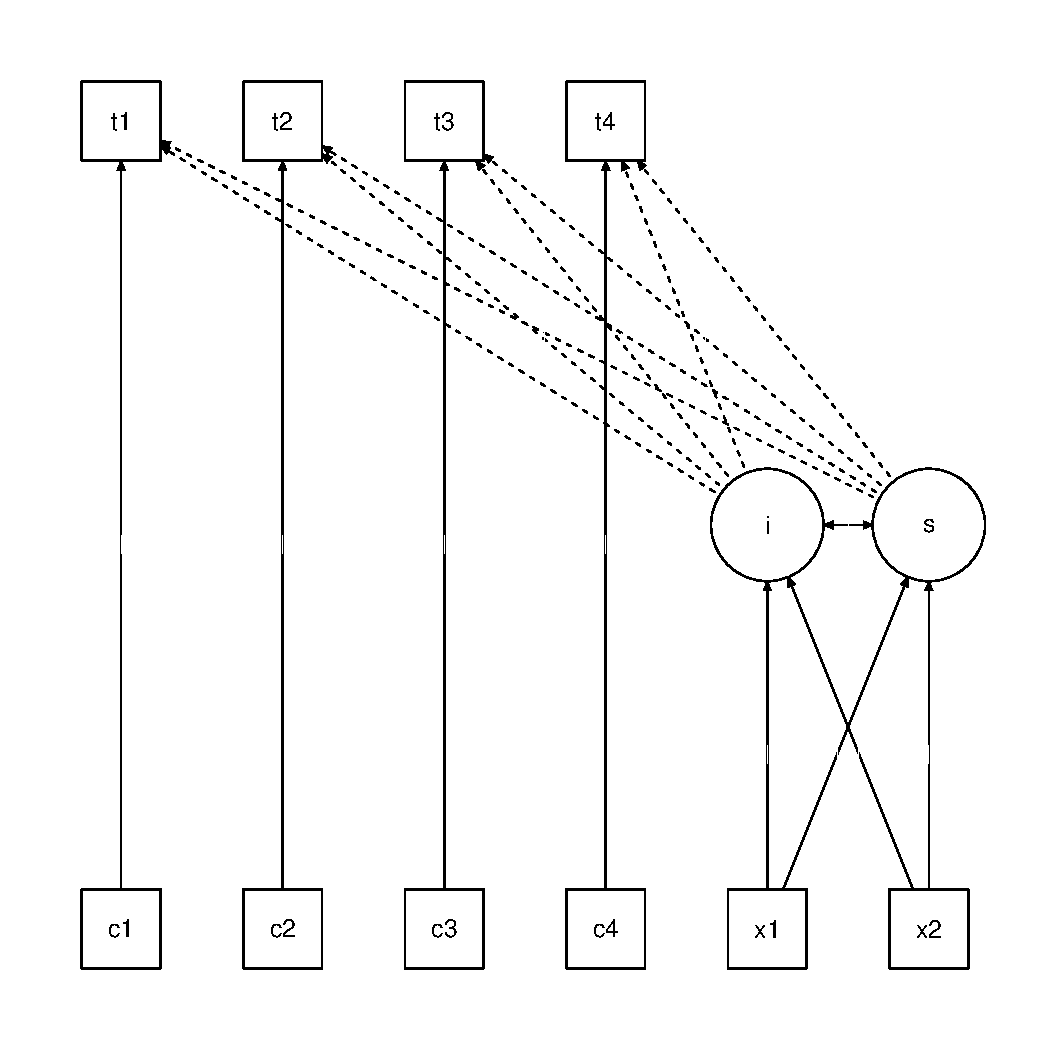
\includegraphics{figure/growth.pdf}

The corresponding syntax is the following:

\begin{verbatim}
# intercept and slope
# with fixed coefficients
  i =~ 1*t1 + 1*t2 + 1*t3 + 1*t4
  s =~ 0*t1 + 1*t2 + 2*t3 + 3*t4
# regressions
  i ~ x1 + x2
  s ~ x1 + x2
# time-varying covariates
  t1 ~ c1
  t2 ~ c2
  t3 ~ c3
  t4 ~ c4
\end{verbatim}

For ease of copy/pasting, the complete R code needed to specify and fit
this linear growth model with a time-varying covariate is printed again
below:

\begin{Shaded}
\begin{Highlighting}[]
\CommentTok{# a linear growth model with a time-varying covariate}
\NormalTok{model <-}\StringTok{ '}
\StringTok{  # intercept and slope with fixed coefficients}
\StringTok{    i =~ 1*t1 + 1*t2 + 1*t3 + 1*t4}
\StringTok{    s =~ 0*t1 + 1*t2 + 2*t3 + 3*t4}
\StringTok{  # regressions}
\StringTok{    i ~ x1 + x2}
\StringTok{    s ~ x1 + x2}
\StringTok{  # time-varying covariates}
\StringTok{    t1 ~ c1}
\StringTok{    t2 ~ c2}
\StringTok{    t3 ~ c3}
\StringTok{    t4 ~ c4}
\StringTok{'}
\NormalTok{fit <-}\StringTok{ }\KeywordTok{growth}\NormalTok{(model, }\DataTypeTok{data =} \NormalTok{Demo.growth)}
\KeywordTok{summary}\NormalTok{(fit)}
\end{Highlighting}
\end{Shaded}


\section{Using categorical variables}
Binary, ordinal and nominal variables are considered categorical (not
continuous). It makes a big difference if these categorical variables
are exogenous (independent) or endogenous (dependent) in the model.

\paragraph{Exogenous categorical variables}

If you have a binary exogenous covariate (say, gender), all you need to
do is to recode it as a dummy (0/1) variable. Just like you would do in
a classic regression model. If you have an exogenous ordinal variable,
you can use a coding scheme reflecting the order (say, 1,2,3,\ldots{})
and treat it as any other (numeric) covariate. If you have a nominal
categorical variable with $K > 2$ levels, you need to replace it by a
set of $K-1$ dummy variables, again, just like you would do in classical
regression.

\paragraph{Endogenous categorical variables}

The lavaan 0.5 series can deal with binary and ordinal (but not nominal)
endogenous variables. Only the three-stage WLS approach is currently
supported, including some `robust' variants. To use binary/ordinal data,
you have two choices:

\begin{enumerate}
\def\labelenumi{\arabic{enumi}.}
\item
  declare them as `ordered' (using the \texttt{ordered} function, which
  is part of base R) in your data.frame before you run the analysis; for
  example, if you need to declare four variables (say, \texttt{item1},
  \texttt{item2}, \texttt{item3}, \texttt{item4}) as ordinal in your
  data.frame (called \texttt{Data}), you can use something like:

\begin{Shaded}
\begin{Highlighting}[]
\NormalTok{Data[,}\KeywordTok{c}\NormalTok{(}\StringTok{"item1"}\NormalTok{,}
        \StringTok{"item2"}\NormalTok{,}
        \StringTok{"item3"}\NormalTok{,}
        \StringTok{"item4"}\NormalTok{)] <-}
\StringTok{    }\KeywordTok{lapply}\NormalTok{(Data[,}\KeywordTok{c}\NormalTok{(}\StringTok{"item1"}\NormalTok{,}
                   \StringTok{"item2"}\NormalTok{,}
                   \StringTok{"item3"}\NormalTok{,}
                   \StringTok{"item4"}\NormalTok{)], ordered)}
\end{Highlighting}
\end{Shaded}
\item
  use the \texttt{ordered} argument when using one of the fitting
  functions (cfa/sem/growth/lavaan), for example, if you have four
  binary or ordinal variables (say, \texttt{item1}, \texttt{item2},
  \texttt{item3}, \texttt{item4}), you can use:

\begin{Shaded}
\begin{Highlighting}[]
\NormalTok{fit <-}\StringTok{ }\KeywordTok{cfa}\NormalTok{(myModel, }\DataTypeTok{data =} \NormalTok{myData,}
           \DataTypeTok{ordered=}\KeywordTok{c}\NormalTok{(}\StringTok{"item1"}\NormalTok{,}\StringTok{"item2"}\NormalTok{,}
                     \StringTok{"item3"}\NormalTok{,}\StringTok{"item4"}\NormalTok{))}
\end{Highlighting}
\end{Shaded}
\end{enumerate}

In both cases, lavaan will automatically switch to the \texttt{WLSMV}
estimator: it will use diagonally weighted least squares (\texttt{DWLS})
to estimate the model parameters, but it will use the full weight matrix
to compute robust standard errors, and a mean- and variance-adjusted
test stastistic.

\section{Using a covariance matrix as input}
If you have no full dataset, but you do have a sample covariance matrix,
you can still fit your model. If you wish to add a mean structure, you
need to provide a mean vector too. Importantly, if only sample
statistics are provided, you must specify the number of observations
that were used to compute the sample moments. The following example
illustrates the use of a sample covariance matrix as input. First, we
read in the lower half of the covariance matrix (including the
diagonal):

\begin{Shaded}
\begin{Highlighting}[]
\NormalTok{lower <-}\StringTok{ '}
\StringTok{ 11.834}
\StringTok{  6.947   9.364}
\StringTok{  6.819   5.091  12.532}
\StringTok{  4.783   5.028   7.495   9.986}
\StringTok{ -3.839  -3.889  -3.841  -3.625  9.610}
\StringTok{-21.899 -18.831 -21.748 -18.775 35.522 450.288 '}

\NormalTok{wheaton.cov <-}\StringTok{ }
\StringTok{    }\KeywordTok{getCov}\NormalTok{(lower, }\DataTypeTok{names =} \KeywordTok{c}\NormalTok{(}\StringTok{"anomia67"}\NormalTok{, }\StringTok{"powerless67"}\NormalTok{, }
                            \StringTok{"anomia71"}\NormalTok{, }\StringTok{"powerless71"}\NormalTok{,}
                            \StringTok{"education"}\NormalTok{, }\StringTok{"sei"}\NormalTok{))}
\end{Highlighting}
\end{Shaded}

The \texttt{getCov()} function makes it easy to create a full covariance
matrix (including variable names) if you only have the lower-half
elements (perhaps pasted from a textbook or a paper). Note that the
lower-half elements are written between two single quotes. Therefore,
you have some additional flexibility. You can add comments, and blank
lines. If the numbers are separated by a comma, or a semi-colon, that is
fine too. For more information about \texttt{getCov()}, see the online
manual page.

Next, we can specify our model, estimate it, and request a summary of
the results:

\begin{Shaded}
\begin{Highlighting}[]
\CommentTok{# classic wheaton et al model}
\NormalTok{wheaton.model <-}\StringTok{ '}
\StringTok{  # latent variables}
\StringTok{    ses     =~ education + sei}
\StringTok{    alien67 =~ anomia67 + powerless67}
\StringTok{    alien71 =~ anomia71 + powerless71}
\StringTok{  # regressions}
\StringTok{    alien71 ~ alien67 + ses}
\StringTok{    alien67 ~ ses}
\StringTok{  # correlated residuals}
\StringTok{    anomia67 ~~ anomia71}
\StringTok{    powerless67 ~~ powerless71}
\StringTok{'}
\NormalTok{fit <-}\StringTok{ }\KeywordTok{sem}\NormalTok{(wheaton.model, }
           \DataTypeTok{sample.cov =} \NormalTok{wheaton.cov, }
           \DataTypeTok{sample.nobs =} \DecValTok{932}\NormalTok{)}
\KeywordTok{summary}\NormalTok{(fit, }\DataTypeTok{standardized =} \OtherTok{TRUE}\NormalTok{)}
\end{Highlighting}
\end{Shaded}

\begin{verbatim}
lavaan (0.5-13) converged normally after  82 iterations

  Number of observations                           932

  Estimator                                         ML
  Minimum Function Test Statistic                4.735
  Degrees of freedom                                 4
  P-value (Chi-square)                           0.316

Parameter estimates:

  Information                                 Expected
  Standard Errors                             Standard

                   Estimate  Std.err  Z-value  P(>|z|)   Std.lv  Std.all
Latent variables:
  ses =~
    education         1.000                               2.607    0.842
    sei               5.219    0.422   12.364    0.000   13.609    0.642
  alien67 =~
    anomia67          1.000                               2.663    0.774
    powerless67       0.979    0.062   15.895    0.000    2.606    0.852
  alien71 =~
    anomia71          1.000                               2.850    0.805
    powerless71       0.922    0.059   15.498    0.000    2.628    0.832

Regressions:
  alien71 ~
    alien67           0.607    0.051   11.898    0.000    0.567    0.567
    ses              -0.227    0.052   -4.334    0.000   -0.207   -0.207
  alien67 ~
    ses              -0.575    0.056  -10.195    0.000   -0.563   -0.563

Covariances:
  anomia67 ~~
    anomia71          1.623    0.314    5.176    0.000    1.623    0.356
  powerless67 ~~
    powerless71       0.339    0.261    1.298    0.194    0.339    0.121

Variances:
    education         2.801    0.507                      2.801    0.292
    sei             264.597   18.126                    264.597    0.588
    anomia67          4.731    0.453                      4.731    0.400
    powerless67       2.563    0.403                      2.563    0.274
    anomia71          4.399    0.515                      4.399    0.351
    powerless71       3.070    0.434                      3.070    0.308
    ses               6.798    0.649                      1.000    1.000
    alien67           4.841    0.467                      0.683    0.683
    alien71           4.083    0.404                      0.503    0.503
\end{verbatim}

If you have multiple groups, the \texttt{sample.cov} argument must be a
list containing the sample variance-covariance matrix of each group as a
separate element in the list. If a mean structure is needed, the
\texttt{sample.mean} argument must be a list containing the sample means
of each group. Finally, the \texttt{sample.nobs} argument can be either
a list or an integer vector containing the number of observations for
each group.

\section{Estimators, standard errors and missing values}
\paragraph{Estimators}

If all data is continuous, the default estimator in the lavaan package
is maximum likelihood (\texttt{estimator = "ML"}). Alternative
estimators available in lavaan are:

\begin{itemize}
\itemsep1pt\parskip0pt\parsep0pt
\item
  \texttt{"GLS"}: generalized least squares. For complete data only.
\item
  \texttt{"WLS"}: weighted least squares (sometimes called ADF
  estimation). For complete data only.
\item
  \texttt{"DWLS"}: diagonally weighted least squares
\item
  \texttt{"ULS"}: unweighted least squares
\end{itemize}

Many estimators have `robust' variants, meaning that they provide robust
standard errors and a scaled test statistic. For example, for the
maximum likelihood estimator, lavaan provides the following robust
variants:

\begin{itemize}
\itemsep1pt\parskip0pt\parsep0pt
\item
  \texttt{"MLM"}: maximum likelihood estimation with robust standard
  errors and a Satorra-Bentler scaled test statistic. For complete data
  only.
\item
  \texttt{"MLMVS"}: maximum likelihood estimation with robust standard
  errors and a mean- and variance adjusted test statistic (aka the
  Satterthwaite approach). For complete data only.
\item
  \texttt{"MLMV"}: maximum likelihood estimation with robust standard
  errors and a mean- and variance adjusted test statistic (using a
  scale-shifted approach). For complete data only.
\item
  \texttt{"MLF"}: for maximum likelihood estimation with standard errors
  based on the first-order derivatives, and a conventional test
  statistic. For both complete and incomplete data.
\item
  \texttt{"MLR"}: maximum likelihood estimation with robust
  (Huber-White) standard errors and a scaled test statistic that is
  (asymptotically) equal to the Yuan-Bentler test statistic. For both
  complete and incomplete data.
\end{itemize}

For the \texttt{DWLS} and \texttt{ULS} estimators, lavaan also provides
`robust' variants: \texttt{WLSM}, \texttt{WLSMVS}, \texttt{WLSMV},
\texttt{ULSM}, \texttt{ULSMVS}, \texttt{ULSMV}. Note that for the robust
\texttt{WLS} variants, we use the diagonal of the weight matrix for
estimation, but we use the full weight matrix to correct the standard
errors and to compute the test statistic.

\paragraph{ML estimation: Wishart versus Normal}

If maximum likelihood estimation is used (\texttt{"ML"} or any of its
robusts variants), the default behavior of lavaan is to base the
analysis on the so-called \emph{biased} sample covariance matrix, where
the elements are divided by $n$ instead of $n-1$. This is done
internally, and should not be done by the user. In addition, the
chi-square statistic is computed by multiplying the minimum function
value with a factor $n$ (instead of $n-1$). This is similar to the Mplus
program. If you prefer to use an unbiased covariance, and $n-1$ as the
multiplier to compute the chi-square statistic, you need to specify the
\texttt{likelihood = "wishart"} argument when calling the fitting
functions. For example:

\begin{Shaded}
\begin{Highlighting}[]
\NormalTok{fit <-}\StringTok{ }\KeywordTok{cfa}\NormalTok{(HS.model, }
           \DataTypeTok{data =} \NormalTok{HolzingerSwineford1939, }
           \DataTypeTok{likelihood =} \StringTok{"wishart"}\NormalTok{)}
\NormalTok{fit}
\end{Highlighting}
\end{Shaded}

\begin{verbatim}
lavaan (0.5-13) converged normally after  41 iterations

  Number of observations                           301

  Estimator                                         ML
  Minimum Function Test Statistic               85.022
  Degrees of freedom                                24
  P-value (Chi-square)                           0.000
\end{verbatim}

The value of the test statistic will be closer to the value reported by
programs like EQS, LISREL or AMOS, since they all use the `Wishart'
approach when using the maximum likelihood estimator. The program Mplus,
on the other hand, uses the `normal' approach to maximum likelihood
estimation.

\paragraph{Missing values}

If the data contain missing values, the default behavior is listwise
deletion. If the missing mechanism is MCAR (missing completely at
random) or MAR (missing at random), the lavaan package provides
case-wise (or `full information') maximum likelihood estimation. You can
turn this feature on, by using the argument \texttt{missing = "ML"} when
calling the fitting function. An unrestricted (h1) model will
automatically be estimated, so that all common fit indices are
available.

\paragraph{Standard errors}

Standard errors are (by default) based on the expected information
matrix. The only exception is when data are missing and full information
ML is used (via \texttt{missing = "ML"}). In this case, the observed
information matrix is used to compute the standard errors. The user can
change this behavior by using the \texttt{information} argument, which
can be set to \texttt{"expected"} or \texttt{"observed"}.

If the estimator is simply \texttt{"ML"}, you can request robust
standard errors by using the \texttt{se} argument, which can be set to
\texttt{"robust.sem"}, \texttt{"robust.huber.white"} ,
\texttt{"first.order"} or \texttt{"bootstrap"}.\\Or simply to
\texttt{"none"} if you don't need them. This will not affect the test
statistic. In fact, you can choose the test statistic independently by
using the \texttt{test} argument, which can be set to
\texttt{"standard"}, \texttt{"Satorra-Bentler"}, \texttt{"Yuan-Bentler"}
or \texttt{"bootstrap"}.

\paragraph{Bootstrapping}

There are two ways for using the bootstrap in lavaan. Either you can set
\texttt{se = "bootstrap"} or \texttt{test = "bootstrap"} when fitting
the model (and you will get bootstrap standard errors, and/or a
bootstrap based p-value respectively), or you can you the
\texttt{boostrapLavaan()} function, which needs an already fitted lavaan
object. The latter function can be used to `bootstrap' any statistic (or
vector of statistics) that you can extract from a fitted lavaan object.

\section{Indirect effects and mediation analysis}
Consider a classical mediation setup with three variables: Y is the
dependent variable, X is the predictor, and M is a mediator. For
illustration, we create a toy dataset containing these three variables,
and fit a path analysis model that includes the direct effect of X on Y
and the indirect effect of X on Y via M.

\begin{Shaded}
\begin{Highlighting}[]
\KeywordTok{set.seed}\NormalTok{(}\DecValTok{1234}\NormalTok{)}
\NormalTok{X <-}\StringTok{ }\KeywordTok{rnorm}\NormalTok{(}\DecValTok{100}\NormalTok{)}
\NormalTok{M <-}\StringTok{ }\FloatTok{0.5}\NormalTok{*X +}\StringTok{ }\KeywordTok{rnorm}\NormalTok{(}\DecValTok{100}\NormalTok{)}
\NormalTok{Y <-}\StringTok{ }\FloatTok{0.7}\NormalTok{*M +}\StringTok{ }\KeywordTok{rnorm}\NormalTok{(}\DecValTok{100}\NormalTok{)}
\NormalTok{Data <-}\StringTok{ }\KeywordTok{data.frame}\NormalTok{(}\DataTypeTok{X =} \NormalTok{X, }\DataTypeTok{Y =} \NormalTok{Y, }\DataTypeTok{M =} \NormalTok{M)}
\NormalTok{model <-}\StringTok{ ' # direct effect}
\StringTok{             Y ~ c*X}
\StringTok{           # mediator}
\StringTok{             M ~ a*X}
\StringTok{             Y ~ b*M}
\StringTok{           # indirect effect (a*b)}
\StringTok{             ab := a*b}
\StringTok{           # total effect}
\StringTok{             total := c + (a*b)}
\StringTok{         '}
\NormalTok{fit <-}\StringTok{ }\KeywordTok{sem}\NormalTok{(model, }\DataTypeTok{data =} \NormalTok{Data)}
\KeywordTok{summary}\NormalTok{(fit)}
\end{Highlighting}
\end{Shaded}

\begin{verbatim}
lavaan (0.5-13) converged normally after  13 iterations

  Number of observations                           100

  Estimator                                         ML
  Minimum Function Test Statistic                0.000
  Degrees of freedom                                 0
  P-value (Chi-square)                           0.000

Parameter estimates:

  Information                                 Expected
  Standard Errors                             Standard

                   Estimate  Std.err  Z-value  P(>|z|)
Regressions:
  Y ~
    X         (c)     0.036    0.104    0.348    0.728
  M ~
    X         (a)     0.474    0.103    4.613    0.000
  Y ~
    M         (b)     0.788    0.092    8.539    0.000

Variances:
    Y                 0.898    0.127
    M                 1.054    0.149

Defined parameters:
    ab                0.374    0.092    4.059    0.000
    total             0.410    0.125    3.287    0.001
\end{verbatim}

The example illustrates the use of the \texttt{":="} operator in the
lavaan model syntax. This operator `defines' new parameters which take
on values that are an arbitrary function of the original model
parameters. The function, however, must be specified in terms of the
parameter \emph{labels} that are explicitly mentioned in the model
syntax. By default, the standard errors for these defined parameters are
computed by using the so-called Delta method. As with other models,
bootstrap standard errors can be requested simply by specifying
\texttt{se = "bootstrap"} in the fitting function.

\section{Modification Indices}
Modification indices can be requested by adding the argument
\texttt{modindices = TRUE} in the \texttt{summary()} call, or by calling
the function \texttt{modindices()} directly. The \texttt{modindices()}
function returns a data frame, which you can sort or filter to extract
what you want. For example, to see only the modification indices for the
factor loadings, you can use something like this:

\begin{Shaded}
\begin{Highlighting}[]
\NormalTok{fit <-}\StringTok{ }\KeywordTok{cfa}\NormalTok{(HS.model, }
           \DataTypeTok{data =} \NormalTok{HolzingerSwineford1939)}
\NormalTok{mi <-}\StringTok{ }\KeywordTok{modindices}\NormalTok{(fit)}
\NormalTok{mi[mi$op ==}\StringTok{ "=~"}\NormalTok{,]}
\end{Highlighting}
\end{Shaded}

\begin{verbatim}
       lhs op rhs     mi    epc sepc.lv sepc.all sepc.nox
1   visual =~  x1     NA     NA      NA       NA       NA
2   visual =~  x2  0.000  0.000   0.000    0.000    0.000
3   visual =~  x3  0.000  0.000   0.000    0.000    0.000
4   visual =~  x4  1.211  0.077   0.069    0.059    0.059
5   visual =~  x5  7.441 -0.210  -0.189   -0.147   -0.147
6   visual =~  x6  2.843  0.111   0.100    0.092    0.092
7   visual =~  x7 18.631 -0.422  -0.380   -0.349   -0.349
8   visual =~  x8  4.295 -0.210  -0.189   -0.187   -0.187
9   visual =~  x9 36.411  0.577   0.519    0.515    0.515
10 textual =~  x1  8.903  0.350   0.347    0.297    0.297
11 textual =~  x2  0.017 -0.011  -0.011   -0.010   -0.010
12 textual =~  x3  9.151 -0.272  -0.269   -0.238   -0.238
13 textual =~  x4     NA     NA      NA       NA       NA
14 textual =~  x5  0.000  0.000   0.000    0.000    0.000
15 textual =~  x6  0.000  0.000   0.000    0.000    0.000
16 textual =~  x7  0.098 -0.021  -0.021   -0.019   -0.019
17 textual =~  x8  3.359 -0.121  -0.120   -0.118   -0.118
18 textual =~  x9  4.796  0.138   0.137    0.136    0.136
19   speed =~  x1  0.014  0.024   0.015    0.013    0.013
20   speed =~  x2  1.580 -0.198  -0.123   -0.105   -0.105
21   speed =~  x3  0.716  0.136   0.084    0.075    0.075
22   speed =~  x4  0.003 -0.005  -0.003   -0.003   -0.003
23   speed =~  x5  0.201 -0.044  -0.027   -0.021   -0.021
24   speed =~  x6  0.273  0.044   0.027    0.025    0.025
25   speed =~  x7     NA     NA      NA       NA       NA
26   speed =~  x8  0.000  0.000   0.000    0.000    0.000
27   speed =~  x9  0.000  0.000   0.000    0.000    0.000
\end{verbatim}

Modification indices are printed out for each nonfree (or nonredundant)
parameter. The modification indices are supplemented by the expected
parameter change (EPC) values (column \texttt{epc}). The last three
columns contain the standardized EPC values (\texttt{sepc.lv}: only
standardizing the latent variables; \texttt{sepc.all}: standardizing all
variables; \texttt{sepc.nox}: standardizing all but exogenous observed
variables)

\section{Extracting information from a fitted model}
The \texttt{summary()} function gives a nice overview of a fitted model,
but is for display only. If you need the actual numbers for further
processing, you may prefer to use one of several `extractor' functions.
We have already seen the \texttt{coef()} function which extracts the
estimated parameters of a fitted model. Other extractor functions are
discussed below.

\paragraph{parameterEstimates}

The \texttt{parameterEstimates} function extracts not only the values of
the estimated parameters, but also the standard errors, the z-values,
the standardized parameter values, and returns everything conveniently
as a data frame. For example:

\begin{Shaded}
\begin{Highlighting}[]
\NormalTok{fit <-}\StringTok{ }\KeywordTok{cfa}\NormalTok{(HS.model, }\DataTypeTok{data =} \NormalTok{HolzingerSwineford1939)}
\KeywordTok{parameterEstimates}\NormalTok{(fit)}
\end{Highlighting}
\end{Shaded}

\begin{verbatim}
       lhs op     rhs   est    se      z pvalue ci.lower ci.upper
1   visual =~      x1 1.000 0.000     NA     NA    1.000    1.000
2   visual =~      x2 0.553 0.100  5.554      0    0.358    0.749
3   visual =~      x3 0.729 0.109  6.685      0    0.516    0.943
4  textual =~      x4 1.000 0.000     NA     NA    1.000    1.000
5  textual =~      x5 1.113 0.065 17.014      0    0.985    1.241
6  textual =~      x6 0.926 0.055 16.703      0    0.817    1.035
7    speed =~      x7 1.000 0.000     NA     NA    1.000    1.000
8    speed =~      x8 1.180 0.165  7.152      0    0.857    1.503
9    speed =~      x9 1.082 0.151  7.155      0    0.785    1.378
10      x1 ~~      x1 0.549 0.114  4.833      0    0.326    0.772
11      x2 ~~      x2 1.134 0.102 11.146      0    0.934    1.333
12      x3 ~~      x3 0.844 0.091  9.317      0    0.667    1.022
13      x4 ~~      x4 0.371 0.048  7.779      0    0.278    0.465
14      x5 ~~      x5 0.446 0.058  7.642      0    0.332    0.561
15      x6 ~~      x6 0.356 0.043  8.277      0    0.272    0.441
16      x7 ~~      x7 0.799 0.081  9.823      0    0.640    0.959
17      x8 ~~      x8 0.488 0.074  6.573      0    0.342    0.633
18      x9 ~~      x9 0.566 0.071  8.003      0    0.427    0.705
19  visual ~~  visual 0.809 0.145  5.564      0    0.524    1.094
20 textual ~~ textual 0.979 0.112  8.737      0    0.760    1.199
21   speed ~~   speed 0.384 0.086  4.451      0    0.215    0.553
22  visual ~~ textual 0.408 0.074  5.552      0    0.264    0.552
23  visual ~~   speed 0.262 0.056  4.660      0    0.152    0.373
24 textual ~~   speed 0.173 0.049  3.518      0    0.077    0.270
\end{verbatim}

\paragraph{standardizedSolution}

The \texttt{standardizedSolution()} function is similar to the
\texttt{parameterEstimates()} function, but only shows the
unstandardized and standardized parameter estimates.

\paragraph{fitted.values}

The \texttt{fitted()} and \texttt{fitted.values()} functions return the
model-implied (fitted) covariance matrix (and mean vector) of a fitted
model:

\begin{Shaded}
\begin{Highlighting}[]
\NormalTok{fit <-}\StringTok{ }\KeywordTok{cfa}\NormalTok{(HS.model, }\DataTypeTok{data =} \NormalTok{HolzingerSwineford1939)}
\KeywordTok{fitted}\NormalTok{(fit)}
\end{Highlighting}
\end{Shaded}

\begin{verbatim}
$cov
   x1    x2    x3    x4    x5    x6    x7    x8    x9   
x1 1.358                                                
x2 0.448 1.382                                          
x3 0.590 0.327 1.275                                    
x4 0.408 0.226 0.298 1.351                              
x5 0.454 0.252 0.331 1.090 1.660                        
x6 0.378 0.209 0.276 0.907 1.010 1.196                  
x7 0.262 0.145 0.191 0.173 0.193 0.161 1.183            
x8 0.309 0.171 0.226 0.205 0.228 0.190 0.453 1.022      
x9 0.284 0.157 0.207 0.188 0.209 0.174 0.415 0.490 1.015

$mean
x1 x2 x3 x4 x5 x6 x7 x8 x9 
 0  0  0  0  0  0  0  0  0 
\end{verbatim}

\paragraph{residuals}

The \texttt{resid()} or \texttt{residuals()} functions return
(unstandardized) residuals of a fitted model. This is simply the
difference between the observed and implied covariance matrix and mean
vector. If the estimator is maximum likelihood, it is also possible to
obtain the normalized and the standardized residuals (note: you may
observe several \texttt{NA} values, but they can be safely ignored)

\begin{Shaded}
\begin{Highlighting}[]
\NormalTok{fit <-}\StringTok{ }\KeywordTok{cfa}\NormalTok{(HS.model, }\DataTypeTok{data =} \NormalTok{HolzingerSwineford1939)}
\KeywordTok{resid}\NormalTok{(fit, }\DataTypeTok{type =} \StringTok{"standardized"}\NormalTok{)}
\end{Highlighting}
\end{Shaded}

\begin{verbatim}
$cov
   x1     x2     x3     x4     x5     x6     x7     x8     x9    
x1     NA                                                        
x2 -2.196     NA                                                 
x3 -1.199  2.692  0.000                                          
x4  2.465 -0.283 -1.948     NA                                   
x5 -0.362 -0.610 -4.443  0.856     NA                            
x6  2.032  0.661 -0.701     NA  0.633     NA                     
x7 -3.787 -3.800 -1.882  0.839 -0.837 -0.321  0.000              
x8 -1.456 -1.137 -0.305 -2.049 -1.100 -0.635  3.804     NA       
x9  4.062  1.517  3.328  1.237  1.723  1.436 -2.772     NA     NA

$mean
x1 x2 x3 x4 x5 x6 x7 x8 x9 
 0  0  0  0  0  0  0  0  0 
\end{verbatim}

\paragraph{vcov}

The function \texttt{vcov()} returns the estimated covariance matrix of
the parameter estimates.

\paragraph{AIC and BIC}

The \texttt{AIC()} and \texttt{BIC()} functions return the AIC and BIC
values of a fitted model.

\paragraph{fitMeasures}

The \texttt{fitMeasures()} function returns all the fit measures
computed by lavaan as a named numeric vector.

\begin{Shaded}
\begin{Highlighting}[]
\NormalTok{fit <-}\StringTok{ }\KeywordTok{cfa}\NormalTok{(HS.model, }\DataTypeTok{data =} \NormalTok{HolzingerSwineford1939)}
\KeywordTok{fitMeasures}\NormalTok{(fit)}
\end{Highlighting}
\end{Shaded}

\begin{verbatim}
             fmin             chisq                df            pvalue 
            0.142            85.306            24.000             0.000 
   baseline.chisq       baseline.df   baseline.pvalue               cfi 
          918.852            36.000             0.000             0.931 
              tli              nnfi               rfi               nfi 
            0.896             0.896             0.861             0.907 
             pnfi               ifi               rni              logl 
            0.605             0.931             0.931         -3737.745 
unrestricted.logl              npar               aic               bic 
        -3695.092            21.000          7517.490          7595.339 
           ntotal              bic2             rmsea    rmsea.ci.lower 
          301.000          7528.739             0.092             0.071 
   rmsea.ci.upper      rmsea.pvalue               rmr        rmr_nomean 
            0.114             0.001             0.082             0.082 
             srmr       srmr_nomean             cn_05             cn_01 
            0.065             0.065           129.490           152.654 
              gfi              agfi              pgfi               mfi 
            0.943             0.894             0.503             0.903 
             ecvi 
            0.423 
\end{verbatim}

If you only want the value of a single fit measure, say, the CFI, you
give the name (in lower case) as the second argument:

\begin{Shaded}
\begin{Highlighting}[]
\NormalTok{fit <-}\StringTok{ }\KeywordTok{cfa}\NormalTok{(HS.model, }\DataTypeTok{data =} \NormalTok{HolzingerSwineford1939)}
\KeywordTok{fitMeasures}\NormalTok{(fit, }\StringTok{"cfi"}\NormalTok{)}
\end{Highlighting}
\end{Shaded}

\begin{verbatim}
  cfi 
0.931 
\end{verbatim}

Or you can provide a vector of fit measures, as in

\begin{Shaded}
\begin{Highlighting}[]
\KeywordTok{fitMeasures}\NormalTok{(fit, }\KeywordTok{c}\NormalTok{(}\StringTok{"cfi"}\NormalTok{, }\StringTok{"rmsea"}\NormalTok{, }\StringTok{"srmr"}\NormalTok{))}
\end{Highlighting}
\end{Shaded}

\begin{verbatim}
  cfi rmsea  srmr 
0.931 0.092 0.065 
\end{verbatim}

\paragraph{inspect}

If you want to peek inside a fitted lavaan object (the object that is
returned by a call to \texttt{cfa()}, \texttt{sem()}or
\texttt{growth()}), you can use the \texttt{inspect()} function, with a
variety of options. By default, calling \texttt{inspect()} on a fitted
lavaan object returns a list of the model matrices that are used
internally to represent the model. The free parameters are nonzero
integers.

\begin{Shaded}
\begin{Highlighting}[]
\NormalTok{fit <-}\StringTok{ }\KeywordTok{cfa}\NormalTok{(HS.model, }\DataTypeTok{data =} \NormalTok{HolzingerSwineford1939)}
\KeywordTok{inspect}\NormalTok{(fit)}
\end{Highlighting}
\end{Shaded}

\begin{verbatim}
$lambda
   visual textul speed
x1      0      0     0
x2      1      0     0
x3      2      0     0
x4      0      0     0
x5      0      3     0
x6      0      4     0
x7      0      0     0
x8      0      0     5
x9      0      0     6

$theta
   x1 x2 x3 x4 x5 x6 x7 x8 x9
x1  7                        
x2  0  8                     
x3  0  0  9                  
x4  0  0  0 10               
x5  0  0  0  0 11            
x6  0  0  0  0  0 12         
x7  0  0  0  0  0  0 13      
x8  0  0  0  0  0  0  0 14   
x9  0  0  0  0  0  0  0  0 15

$psi
        visual textul speed
visual  16                 
textual 19     17          
speed   20     21     18   
\end{verbatim}

To see the starting values of parameters in each model matrix, type

\begin{Shaded}
\begin{Highlighting}[]
\KeywordTok{inspect}\NormalTok{(fit, }\DataTypeTok{what =} \StringTok{"start"}\NormalTok{)}
\end{Highlighting}
\end{Shaded}

\begin{verbatim}
$lambda
   visual textul speed
x1  1.000  0.000 0.000
x2  0.778  0.000 0.000
x3  1.107  0.000 0.000
x4  0.000  1.000 0.000
x5  0.000  1.133 0.000
x6  0.000  0.924 0.000
x7  0.000  0.000 1.000
x8  0.000  0.000 1.225
x9  0.000  0.000 0.854

$theta
   x1    x2    x3    x4    x5    x6    x7    x8    x9   
x1 0.679                                                
x2 0.000 0.691                                          
x3 0.000 0.000 0.637                                    
x4 0.000 0.000 0.000 0.675                              
x5 0.000 0.000 0.000 0.000 0.830                        
x6 0.000 0.000 0.000 0.000 0.000 0.598                  
x7 0.000 0.000 0.000 0.000 0.000 0.000 0.592            
x8 0.000 0.000 0.000 0.000 0.000 0.000 0.000 0.511      
x9 0.000 0.000 0.000 0.000 0.000 0.000 0.000 0.000 0.508

$psi
        visual textul speed
visual  0.05               
textual 0.00   0.05        
speed   0.00   0.00   0.05 
\end{verbatim}

To see how lavaan internally represents a model, you can type

\begin{Shaded}
\begin{Highlighting}[]
\KeywordTok{inspect}\NormalTok{(fit, }\DataTypeTok{what =} \StringTok{"list"}\NormalTok{)}
\end{Highlighting}
\end{Shaded}

\begin{verbatim}
   id     lhs op     rhs user group free ustart exo label eq.id unco
1   1  visual =~      x1    1     1    0      1   0           0    0
2   2  visual =~      x2    1     1    1     NA   0           0    1
3   3  visual =~      x3    1     1    2     NA   0           0    2
4   4 textual =~      x4    1     1    0      1   0           0    0
5   5 textual =~      x5    1     1    3     NA   0           0    3
6   6 textual =~      x6    1     1    4     NA   0           0    4
7   7   speed =~      x7    1     1    0      1   0           0    0
8   8   speed =~      x8    1     1    5     NA   0           0    5
9   9   speed =~      x9    1     1    6     NA   0           0    6
10 10      x1 ~~      x1    0     1    7     NA   0           0    7
11 11      x2 ~~      x2    0     1    8     NA   0           0    8
12 12      x3 ~~      x3    0     1    9     NA   0           0    9
13 13      x4 ~~      x4    0     1   10     NA   0           0   10
14 14      x5 ~~      x5    0     1   11     NA   0           0   11
15 15      x6 ~~      x6    0     1   12     NA   0           0   12
16 16      x7 ~~      x7    0     1   13     NA   0           0   13
17 17      x8 ~~      x8    0     1   14     NA   0           0   14
18 18      x9 ~~      x9    0     1   15     NA   0           0   15
19 19  visual ~~  visual    0     1   16     NA   0           0   16
20 20 textual ~~ textual    0     1   17     NA   0           0   17
21 21   speed ~~   speed    0     1   18     NA   0           0   18
22 22  visual ~~ textual    0     1   19     NA   0           0   19
23 23  visual ~~   speed    0     1   20     NA   0           0   20
24 24 textual ~~   speed    0     1   21     NA   0           0   21
\end{verbatim}

This is equivalent to the \texttt{parTable(fit)} function. The table
that is returned here is called the `parameter table'.

For more inspect options, see the help page for the lavaan class which
you can find by typing the following:

\begin{Shaded}
\begin{Highlighting}[]
\NormalTok{class?lavaan}
\end{Highlighting}
\end{Shaded}


\end{document}
